\documentclass[twoside]{book}

% Packages required by doxygen
\usepackage{fixltx2e}
\usepackage{calc}
\usepackage{doxygen}
\usepackage[export]{adjustbox} % also loads graphicx
\usepackage{graphicx}
\usepackage[utf8]{inputenc}
\usepackage{makeidx}
\usepackage{multicol}
\usepackage{multirow}
\PassOptionsToPackage{warn}{textcomp}
\usepackage{textcomp}
\usepackage[nointegrals]{wasysym}
\usepackage[table]{xcolor}

% Font selection
\usepackage[T1]{fontenc}
\usepackage[scaled=.90]{helvet}
\usepackage{courier}
\usepackage{amssymb}
\usepackage{sectsty}
\renewcommand{\familydefault}{\sfdefault}
\allsectionsfont{%
  \fontseries{bc}\selectfont%
  \color{darkgray}%
}
\renewcommand{\DoxyLabelFont}{%
  \fontseries{bc}\selectfont%
  \color{darkgray}%
}
\newcommand{\+}{\discretionary{\mbox{\scriptsize$\hookleftarrow$}}{}{}}

% Page & text layout
\usepackage{geometry}
\geometry{%
  a4paper,%
  top=2.5cm,%
  bottom=2.5cm,%
  left=2.5cm,%
  right=2.5cm%
}
\tolerance=750
\hfuzz=15pt
\hbadness=750
\setlength{\emergencystretch}{15pt}
\setlength{\parindent}{0cm}
\setlength{\parskip}{3ex plus 2ex minus 2ex}
\makeatletter
\renewcommand{\paragraph}{%
  \@startsection{paragraph}{4}{0ex}{-1.0ex}{1.0ex}{%
    \normalfont\normalsize\bfseries\SS@parafont%
  }%
}
\renewcommand{\subparagraph}{%
  \@startsection{subparagraph}{5}{0ex}{-1.0ex}{1.0ex}{%
    \normalfont\normalsize\bfseries\SS@subparafont%
  }%
}
\makeatother

% Headers & footers
\usepackage{fancyhdr}
\pagestyle{fancyplain}
\fancyhead[LE]{\fancyplain{}{\bfseries\thepage}}
\fancyhead[CE]{\fancyplain{}{}}
\fancyhead[RE]{\fancyplain{}{\bfseries\leftmark}}
\fancyhead[LO]{\fancyplain{}{\bfseries\rightmark}}
\fancyhead[CO]{\fancyplain{}{}}
\fancyhead[RO]{\fancyplain{}{\bfseries\thepage}}
\fancyfoot[LE]{\fancyplain{}{}}
\fancyfoot[CE]{\fancyplain{}{}}
\fancyfoot[RE]{\fancyplain{}{\bfseries\scriptsize Generated by Doxygen }}
\fancyfoot[LO]{\fancyplain{}{\bfseries\scriptsize Generated by Doxygen }}
\fancyfoot[CO]{\fancyplain{}{}}
\fancyfoot[RO]{\fancyplain{}{}}
\renewcommand{\footrulewidth}{0.4pt}
\renewcommand{\chaptermark}[1]{%
  \markboth{#1}{}%
}
\renewcommand{\sectionmark}[1]{%
  \markright{\thesection\ #1}%
}

% Indices & bibliography
\usepackage{natbib}
\usepackage[titles]{tocloft}
\setcounter{tocdepth}{3}
\setcounter{secnumdepth}{5}
\makeindex

% Hyperlinks (required, but should be loaded last)
\usepackage{ifpdf}
\ifpdf
  \usepackage[pdftex,pagebackref=true]{hyperref}
\else
  \usepackage[ps2pdf,pagebackref=true]{hyperref}
\fi
\hypersetup{%
  colorlinks=true,%
  linkcolor=blue,%
  citecolor=blue,%
  unicode%
}

% Custom commands
\newcommand{\clearemptydoublepage}{%
  \newpage{\pagestyle{empty}\cleardoublepage}%
}

\usepackage{caption}
\captionsetup{labelsep=space,justification=centering,font={bf},singlelinecheck=off,skip=4pt,position=top}

%===== C O N T E N T S =====

\begin{document}

% Titlepage & ToC
\hypersetup{pageanchor=false,
             bookmarksnumbered=true,
             pdfencoding=unicode
            }
\pagenumbering{roman}
\begin{titlepage}
\vspace*{7cm}
\begin{center}%
{\Large c-\/chat }\\
\vspace*{1cm}
{\large Generated by Doxygen 1.8.11}\\
\end{center}
\end{titlepage}
\clearemptydoublepage
\tableofcontents
\clearemptydoublepage
\pagenumbering{arabic}
\hypersetup{pageanchor=true}

%--- Begin generated contents ---
\chapter{c-\/chat}
\label{index}\hypertarget{index}{}c-\/chat is a simple terminal chat program for G\+N\+U/\+Linux and i\+OS.

It allows a fairly large number of users to exchange text messages through a client/server architecture. The project wants to be a simple, minimal alternative to popular chat services used in the workplace or to discuss common interests.

The implementation is entirely in C to keep the program efficient and small.

\subsection*{Structure}

The source files directory contains 3 subdirectories\+:


\begin{DoxyItemize}
\item client -\/ containing the source code for the client application.
\item server -\/ containing the source code for the server application.
\item util -\/ containing libraries and headers used in both the executables.
\end{DoxyItemize}

For further information refer to the documents in the \char`\"{}report/\char`\"{} directory. 
\chapter{Data Structure Index}
\section{Data Structures}
Here are the data structures with brief descriptions\+:\begin{DoxyCompactList}
\item\contentsline{section}{\hyperlink{structClientInfo}{Client\+Info} \\*Structure containing the informations regarding a single connection with a client }{\pageref{structClientInfo}}{}
\item\contentsline{section}{\hyperlink{structLinkedList}{Linked\+List} \\*Linked list structure }{\pageref{structLinkedList}}{}
\item\contentsline{section}{\hyperlink{structLLNode}{L\+L\+Node} \\*Node of the linked list, representing a connection }{\pageref{structLLNode}}{}
\item\contentsline{section}{\hyperlink{structPacket}{Packet} \\*Structure representing a single packet exchanged between the server and the clients }{\pageref{structPacket}}{}
\end{DoxyCompactList}

\chapter{File Index}
\section{File List}
Here is a list of all documented files with brief descriptions\+:\begin{DoxyCompactList}
\item\contentsline{section}{src/client/\hyperlink{client_8c}{client.\+c} \\*Client chat application for the c-\/chat project }{\pageref{client_8c}}{}
\item\contentsline{section}{src/client/\hyperlink{client_8h}{client.\+h} \\*Client chat application for the c-\/chat project }{\pageref{client_8h}}{}
\item\contentsline{section}{src/server/\hyperlink{clientlist_8c}{clientlist.\+c} \\*Linked list implementation where every node represent a connection with a client }{\pageref{clientlist_8c}}{}
\item\contentsline{section}{src/server/\hyperlink{clientlist_8h}{clientlist.\+h} \\*Linked list implementation where every node represent a connection with a client }{\pageref{clientlist_8h}}{}
\item\contentsline{section}{src/server/\hyperlink{server_8c}{server.\+c} \\*Server chat application for the c-\/chat project }{\pageref{server_8c}}{}
\item\contentsline{section}{src/server/\hyperlink{server_8h}{server.\+h} \\*Server chat application for the c-\/chat project }{\pageref{server_8h}}{}
\item\contentsline{section}{src/util/\hyperlink{networkdef_8h}{networkdef.\+h} \\*Parameters, structures and definitions relative to the applications\textquotesingle{} behaviour and the connection\textquotesingle{}s protocol }{\pageref{networkdef_8h}}{}
\item\contentsline{section}{src/util/\hyperlink{networkutil_8c}{networkutil.\+c} \\*Collection of utility methods used in the c-\/chat project }{\pageref{networkutil_8c}}{}
\item\contentsline{section}{src/util/\hyperlink{networkutil_8h}{networkutil.\+h} \\*Collection of utility methods used in the c-\/chat project }{\pageref{networkutil_8h}}{}
\end{DoxyCompactList}

\chapter{Data Structure Documentation}
\hypertarget{structClientInfo}{}\section{Client\+Info Struct Reference}
\label{structClientInfo}\index{Client\+Info@{Client\+Info}}


Structure containing the informations regarding a single connection with a client.  




{\ttfamily \#include $<$networkdef.\+h$>$}

\subsection*{Data Fields}
\begin{DoxyCompactItemize}
\item 
pthread\+\_\+t \hyperlink{structClientInfo_a473c67886fcb2ae0b18b04e6890870ba}{thread\+\_\+\+ID}
\item 
int \hyperlink{structClientInfo_a2e6d4c5d276144166df3a511592b9c49}{sockfd}
\item 
char \hyperlink{structClientInfo_abeb73c8567e22ae0d8b01f51e08b3260}{alias} \mbox{[}\hyperlink{networkdef_8h_aa07ba58ae52cf11992b7e112454a3eea}{A\+L\+I\+A\+S\+L\+EN}\mbox{]}
\end{DoxyCompactItemize}


\subsection{Detailed Description}
Structure containing the informations regarding a single connection with a client. 

This structure is used by the server application 

\subsection{Field Documentation}
\index{Client\+Info@{Client\+Info}!alias@{alias}}
\index{alias@{alias}!Client\+Info@{Client\+Info}}
\subsubsection[{\texorpdfstring{alias}{alias}}]{\setlength{\rightskip}{0pt plus 5cm}Client\+Info\+::alias}\hypertarget{structClientInfo_abeb73c8567e22ae0d8b01f51e08b3260}{}\label{structClientInfo_abeb73c8567e22ae0d8b01f51e08b3260}
Alias of the client associated to this connection. \index{Client\+Info@{Client\+Info}!sockfd@{sockfd}}
\index{sockfd@{sockfd}!Client\+Info@{Client\+Info}}
\subsubsection[{\texorpdfstring{sockfd}{sockfd}}]{\setlength{\rightskip}{0pt plus 5cm}Client\+Info\+::sockfd}\hypertarget{structClientInfo_a2e6d4c5d276144166df3a511592b9c49}{}\label{structClientInfo_a2e6d4c5d276144166df3a511592b9c49}
Socket file descriptor associated with this connection. \index{Client\+Info@{Client\+Info}!thread\+\_\+\+ID@{thread\+\_\+\+ID}}
\index{thread\+\_\+\+ID@{thread\+\_\+\+ID}!Client\+Info@{Client\+Info}}
\subsubsection[{\texorpdfstring{thread\+\_\+\+ID}{thread_ID}}]{\setlength{\rightskip}{0pt plus 5cm}Client\+Info\+::thread\+\_\+\+ID}\hypertarget{structClientInfo_a473c67886fcb2ae0b18b04e6890870ba}{}\label{structClientInfo_a473c67886fcb2ae0b18b04e6890870ba}
Pointer to the server\textquotesingle{}s thread associated to this connection. 

The documentation for this struct was generated from the following file\+:\begin{DoxyCompactItemize}
\item 
src/util/\hyperlink{networkdef_8h}{networkdef.\+h}\end{DoxyCompactItemize}

\hypertarget{structLinkedList}{}\section{Linked\+List Struct Reference}
\label{structLinkedList}\index{Linked\+List@{Linked\+List}}


Linked list structure.  




{\ttfamily \#include $<$clientlist.\+h$>$}



Collaboration diagram for Linked\+List\+:\nopagebreak
\begin{figure}[H]
\begin{center}
\leavevmode
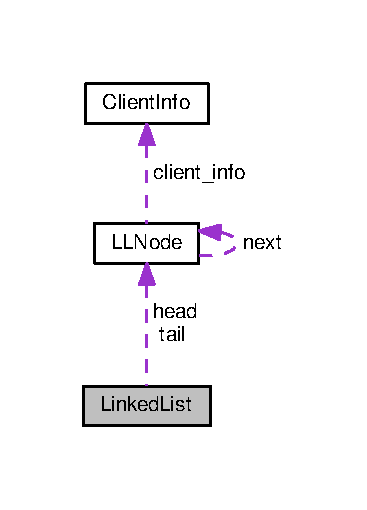
\includegraphics[width=176pt]{structLinkedList__coll__graph}
\end{center}
\end{figure}
\subsection*{Data Fields}
\begin{DoxyCompactItemize}
\item 
struct \hyperlink{structLLNode}{L\+L\+Node} $\ast$ \hyperlink{structLinkedList_a6bcf92a302661a0ef84d2ce766b73136}{head}
\item 
struct \hyperlink{structLLNode}{L\+L\+Node} $\ast$ \hyperlink{structLinkedList_a18d79a06868a03b79f30ebf650f7379d}{tail}
\item 
int \hyperlink{structLinkedList_a4c3f611f9904b8b0f10a374426e59b5d}{size}
\end{DoxyCompactItemize}


\subsection{Detailed Description}
Linked list structure. 

\subsection{Field Documentation}
\index{Linked\+List@{Linked\+List}!head@{head}}
\index{head@{head}!Linked\+List@{Linked\+List}}
\subsubsection[{\texorpdfstring{head}{head}}]{\setlength{\rightskip}{0pt plus 5cm}Linked\+List\+::head}\hypertarget{structLinkedList_a6bcf92a302661a0ef84d2ce766b73136}{}\label{structLinkedList_a6bcf92a302661a0ef84d2ce766b73136}
Pointer to the first node of the list. \index{Linked\+List@{Linked\+List}!size@{size}}
\index{size@{size}!Linked\+List@{Linked\+List}}
\subsubsection[{\texorpdfstring{size}{size}}]{\setlength{\rightskip}{0pt plus 5cm}Linked\+List\+::size}\hypertarget{structLinkedList_a4c3f611f9904b8b0f10a374426e59b5d}{}\label{structLinkedList_a4c3f611f9904b8b0f10a374426e59b5d}
Number of nodes in the list. \index{Linked\+List@{Linked\+List}!tail@{tail}}
\index{tail@{tail}!Linked\+List@{Linked\+List}}
\subsubsection[{\texorpdfstring{tail}{tail}}]{\setlength{\rightskip}{0pt plus 5cm}Linked\+List\+::tail}\hypertarget{structLinkedList_a18d79a06868a03b79f30ebf650f7379d}{}\label{structLinkedList_a18d79a06868a03b79f30ebf650f7379d}
Pointer to the last node of the list. 

The documentation for this struct was generated from the following file\+:\begin{DoxyCompactItemize}
\item 
src/server/\hyperlink{clientlist_8h}{clientlist.\+h}\end{DoxyCompactItemize}

\hypertarget{structLLNode}{}\section{L\+L\+Node Struct Reference}
\label{structLLNode}\index{L\+L\+Node@{L\+L\+Node}}


Node of the linked list, representing a connection.  




{\ttfamily \#include $<$clientlist.\+h$>$}



Collaboration diagram for L\+L\+Node\+:\nopagebreak
\begin{figure}[H]
\begin{center}
\leavevmode
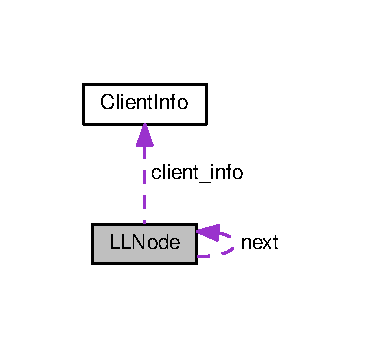
\includegraphics[width=175pt]{structLLNode__coll__graph}
\end{center}
\end{figure}
\subsection*{Data Fields}
\begin{DoxyCompactItemize}
\item 
struct \hyperlink{structClientInfo}{Client\+Info} \hyperlink{structLLNode_ab4552dd6aa88846b769ed067679858c4}{client\+\_\+info}
\item 
struct \hyperlink{structLLNode}{L\+L\+Node} $\ast$ \hyperlink{structLLNode_a55f6432e4bb952037758122d032aaaf2}{next}
\end{DoxyCompactItemize}


\subsection{Detailed Description}
Node of the linked list, representing a connection. 

\subsection{Field Documentation}
\index{L\+L\+Node@{L\+L\+Node}!client\+\_\+info@{client\+\_\+info}}
\index{client\+\_\+info@{client\+\_\+info}!L\+L\+Node@{L\+L\+Node}}
\subsubsection[{\texorpdfstring{client\+\_\+info}{client_info}}]{\setlength{\rightskip}{0pt plus 5cm}L\+L\+Node\+::client\+\_\+info}\hypertarget{structLLNode_ab4552dd6aa88846b769ed067679858c4}{}\label{structLLNode_ab4552dd6aa88846b769ed067679858c4}
{\ttfamily \hyperlink{structClientInfo}{Client\+Info}} struct containing the actual informations. \index{L\+L\+Node@{L\+L\+Node}!next@{next}}
\index{next@{next}!L\+L\+Node@{L\+L\+Node}}
\subsubsection[{\texorpdfstring{next}{next}}]{\setlength{\rightskip}{0pt plus 5cm}L\+L\+Node\+::next}\hypertarget{structLLNode_a55f6432e4bb952037758122d032aaaf2}{}\label{structLLNode_a55f6432e4bb952037758122d032aaaf2}
Pointer to the next node of the list. 

The documentation for this struct was generated from the following file\+:\begin{DoxyCompactItemize}
\item 
src/server/\hyperlink{clientlist_8h}{clientlist.\+h}\end{DoxyCompactItemize}

\hypertarget{structPacket}{}\section{Packet Struct Reference}
\label{structPacket}\index{Packet@{Packet}}


Structure representing a single packet exchanged between the server and the clients.  




{\ttfamily \#include $<$networkdef.\+h$>$}

\subsection*{Data Fields}
\begin{DoxyCompactItemize}
\item 
unsigned char \hyperlink{structPacket_a41917e52ffd1d92b7477073cbbceddee}{action}
\item 
char \hyperlink{structPacket_ac20e801b8bbe165a85317fc937d11cf3}{alias} \mbox{[}\hyperlink{networkdef_8h_aa07ba58ae52cf11992b7e112454a3eea}{A\+L\+I\+A\+S\+L\+EN}\mbox{]}
\item 
int \hyperlink{structPacket_a1d26d154760776ebcea98638b0bf1f73}{len}
\item 
char \hyperlink{structPacket_a819db228469a8fd8beb62114dbfaed56}{payload} \mbox{[}\hyperlink{networkdef_8h_a2ec728de0089ed37af934ae60ed1cd7f}{P\+A\+Y\+L\+EN}\mbox{]}
\end{DoxyCompactItemize}


\subsection{Detailed Description}
Structure representing a single packet exchanged between the server and the clients. 

\subsection{Field Documentation}
\index{Packet@{Packet}!action@{action}}
\index{action@{action}!Packet@{Packet}}
\subsubsection[{\texorpdfstring{action}{action}}]{\setlength{\rightskip}{0pt plus 5cm}Packet\+::action}\hypertarget{structPacket_a41917e52ffd1d92b7477073cbbceddee}{}\label{structPacket_a41917e52ffd1d92b7477073cbbceddee}
Action code of this packet. The possible values can be found in the definitions of the file {\ttfamily \hyperlink{networkdef_8h}{networkdef.\+h}} \index{Packet@{Packet}!alias@{alias}}
\index{alias@{alias}!Packet@{Packet}}
\subsubsection[{\texorpdfstring{alias}{alias}}]{\setlength{\rightskip}{0pt plus 5cm}Packet\+::alias}\hypertarget{structPacket_ac20e801b8bbe165a85317fc937d11cf3}{}\label{structPacket_ac20e801b8bbe165a85317fc937d11cf3}
Field that can contain an alias. Its use is explained in the protocol description. \index{Packet@{Packet}!len@{len}}
\index{len@{len}!Packet@{Packet}}
\subsubsection[{\texorpdfstring{len}{len}}]{\setlength{\rightskip}{0pt plus 5cm}Packet\+::len}\hypertarget{structPacket_a1d26d154760776ebcea98638b0bf1f73}{}\label{structPacket_a1d26d154760776ebcea98638b0bf1f73}
Field that can contain an integer. Its use is explained in the protocol description. \index{Packet@{Packet}!payload@{payload}}
\index{payload@{payload}!Packet@{Packet}}
\subsubsection[{\texorpdfstring{payload}{payload}}]{\setlength{\rightskip}{0pt plus 5cm}Packet\+::payload}\hypertarget{structPacket_a819db228469a8fd8beb62114dbfaed56}{}\label{structPacket_a819db228469a8fd8beb62114dbfaed56}
\hyperlink{structPacket}{Packet}\textquotesingle{}s main body. 

The documentation for this struct was generated from the following file\+:\begin{DoxyCompactItemize}
\item 
src/util/\hyperlink{networkdef_8h}{networkdef.\+h}\end{DoxyCompactItemize}

\chapter{File Documentation}
\hypertarget{client_8c}{}\section{src/client/client.c File Reference}
\label{client_8c}\index{src/client/client.\+c@{src/client/client.\+c}}


Client chat application for the c-\/chat project.  


{\ttfamily \#include \char`\"{}client.\+h\char`\"{}}\\*
{\ttfamily \#include \char`\"{}networkdef.\+h\char`\"{}}\\*
{\ttfamily \#include \char`\"{}networkutil.\+h\char`\"{}}\\*
{\ttfamily \#include $<$stdio.\+h$>$}\\*
{\ttfamily \#include $<$stdlib.\+h$>$}\\*
{\ttfamily \#include $<$unistd.\+h$>$}\\*
{\ttfamily \#include $<$errno.\+h$>$}\\*
{\ttfamily \#include $<$string.\+h$>$}\\*
{\ttfamily \#include $<$netdb.\+h$>$}\\*
{\ttfamily \#include $<$sys/types.\+h$>$}\\*
{\ttfamily \#include $<$netinet/in.\+h$>$}\\*
{\ttfamily \#include $<$sys/socket.\+h$>$}\\*
{\ttfamily \#include $<$arpa/inet.\+h$>$}\\*
{\ttfamily \#include $<$pthread.\+h$>$}\\*
Include dependency graph for client.\+c\+:\nopagebreak
\begin{figure}[H]
\begin{center}
\leavevmode
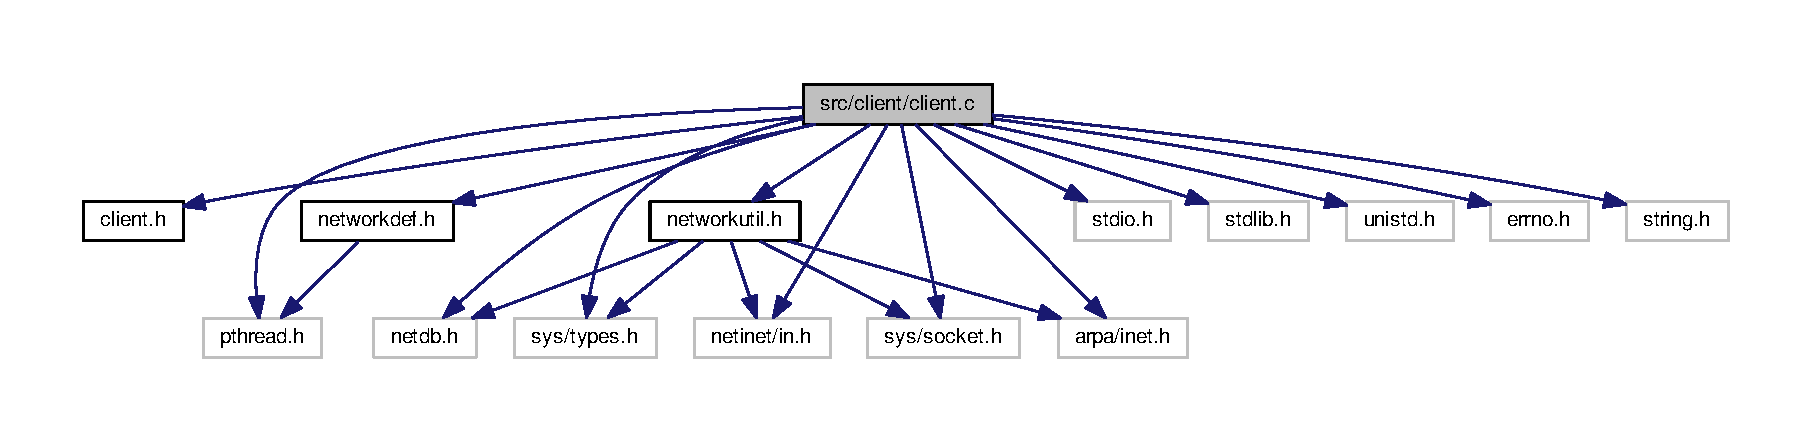
\includegraphics[width=350pt]{client_8c__incl}
\end{center}
\end{figure}
\subsection*{Functions}
\begin{DoxyCompactItemize}
\item 
int {\bfseries main} (int argc, char $\ast$argv\mbox{[}$\,$\mbox{]})\hypertarget{client_8c_a0ddf1224851353fc92bfbff6f499fa97}{}\label{client_8c_a0ddf1224851353fc92bfbff6f499fa97}

\end{DoxyCompactItemize}
\subsection*{Variables}
\begin{DoxyCompactItemize}
\item 
int \hyperlink{client_8c_a9709aefe4930807392898aecb0cb8a79}{connected}
\item 
int \hyperlink{client_8c_a09fb4aa8720896dcbcbe5cece1bfeb27}{serversfd}
\item 
char \hyperlink{client_8c_a62c5d73d188a0bea504be16faa96e5a2}{myalias} \mbox{[}\hyperlink{networkdef_8h_aa07ba58ae52cf11992b7e112454a3eea}{A\+L\+I\+A\+S\+L\+EN}\mbox{]}
\item 
char \hyperlink{client_8c_a77e4114b1f1d4373537d8da2d3ed2e78}{server\+\_\+ip} \mbox{[}I\+N\+E\+T6\+\_\+\+A\+D\+D\+R\+S\+T\+R\+L\+EN\mbox{]}
\item 
char \hyperlink{client_8c_ae7c766edbee46e012d2f333f725d3d37}{server\+\_\+port} \mbox{[}6\mbox{]}
\end{DoxyCompactItemize}


\subsection{Detailed Description}
Client chat application for the c-\/chat project. 

\begin{DoxyAuthor}{Author}
Enrico Vianello (\href{mailto:enrico.vianello.1@studenti.unipd.it}{\tt enrico.\+vianello.\+1@studenti.\+unipd.\+it}) 
\end{DoxyAuthor}
\begin{DoxyVersion}{Version}
1.\+0 
\end{DoxyVersion}
\begin{DoxySince}{Since}
1.\+0
\end{DoxySince}
\begin{DoxyCopyright}{Copyright}
Copyright (c) 2016-\/2017, Enrico Vianello 
\end{DoxyCopyright}


\subsection{Variable Documentation}
\index{client.\+c@{client.\+c}!connected@{connected}}
\index{connected@{connected}!client.\+c@{client.\+c}}
\subsubsection[{\texorpdfstring{connected}{connected}}]{\setlength{\rightskip}{0pt plus 5cm}int connected}\hypertarget{client_8c_a9709aefe4930807392898aecb0cb8a79}{}\label{client_8c_a9709aefe4930807392898aecb0cb8a79}
Connection status\+: 1 if connected with a server, 0 elsewhere \index{client.\+c@{client.\+c}!myalias@{myalias}}
\index{myalias@{myalias}!client.\+c@{client.\+c}}
\subsubsection[{\texorpdfstring{myalias}{myalias}}]{\setlength{\rightskip}{0pt plus 5cm}char myalias\mbox{[}{\bf A\+L\+I\+A\+S\+L\+EN}\mbox{]}}\hypertarget{client_8c_a62c5d73d188a0bea504be16faa96e5a2}{}\label{client_8c_a62c5d73d188a0bea504be16faa96e5a2}
Alias of the client \index{client.\+c@{client.\+c}!server\+\_\+ip@{server\+\_\+ip}}
\index{server\+\_\+ip@{server\+\_\+ip}!client.\+c@{client.\+c}}
\subsubsection[{\texorpdfstring{server\+\_\+ip}{server_ip}}]{\setlength{\rightskip}{0pt plus 5cm}char server\+\_\+ip\mbox{[}I\+N\+E\+T6\+\_\+\+A\+D\+D\+R\+S\+T\+R\+L\+EN\mbox{]}}\hypertarget{client_8c_a77e4114b1f1d4373537d8da2d3ed2e78}{}\label{client_8c_a77e4114b1f1d4373537d8da2d3ed2e78}
Server\textquotesingle{}s IP \index{client.\+c@{client.\+c}!server\+\_\+port@{server\+\_\+port}}
\index{server\+\_\+port@{server\+\_\+port}!client.\+c@{client.\+c}}
\subsubsection[{\texorpdfstring{server\+\_\+port}{server_port}}]{\setlength{\rightskip}{0pt plus 5cm}char server\+\_\+port\mbox{[}6\mbox{]}}\hypertarget{client_8c_ae7c766edbee46e012d2f333f725d3d37}{}\label{client_8c_ae7c766edbee46e012d2f333f725d3d37}
Server\textquotesingle{}s port \index{client.\+c@{client.\+c}!serversfd@{serversfd}}
\index{serversfd@{serversfd}!client.\+c@{client.\+c}}
\subsubsection[{\texorpdfstring{serversfd}{serversfd}}]{\setlength{\rightskip}{0pt plus 5cm}int serversfd}\hypertarget{client_8c_a09fb4aa8720896dcbcbe5cece1bfeb27}{}\label{client_8c_a09fb4aa8720896dcbcbe5cece1bfeb27}
Socket file descriptor of the connection with the server 
\hypertarget{client_8h}{}\section{src/client/client.h File Reference}
\label{client_8h}\index{src/client/client.\+h@{src/client/client.\+h}}


Client chat application for the c-\/chat project.  


This graph shows which files directly or indirectly include this file\+:\nopagebreak
\begin{figure}[H]
\begin{center}
\leavevmode
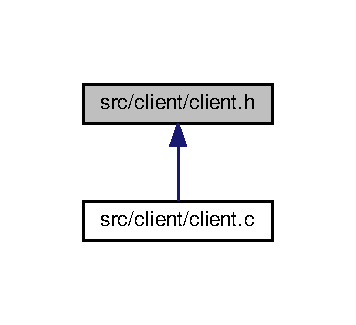
\includegraphics[width=171pt]{client_8h__dep__incl}
\end{center}
\end{figure}
\subsection*{Macros}
\begin{DoxyCompactItemize}
\item 
\#define \hyperlink{client_8h_a137aa83ec74421d226a90c92ec032ac9}{K\+N\+RM}~\char`\"{}\textbackslash{}x1B\mbox{[}0m\char`\"{}
\item 
\#define \hyperlink{client_8h_a66290957baed5df3930ada4cb8caccf1}{K\+R\+ED}~\char`\"{}\textbackslash{}x1B\mbox{[}31m\char`\"{}
\item 
\#define \hyperlink{client_8h_ac081c83b067273757f7a2e54a5957d41}{K\+G\+RN}~\char`\"{}\textbackslash{}x1B\mbox{[}32m\char`\"{}
\item 
\#define \hyperlink{client_8h_a897b10d246533c95ba86cb79f92e465a}{K\+Y\+EL}~\char`\"{}\textbackslash{}x1B\mbox{[}33m\char`\"{}
\item 
\#define \hyperlink{client_8h_a3f838f2fc3a9a3b434be606fc908964b}{K\+B\+LU}~\char`\"{}\textbackslash{}x1B\mbox{[}34m\char`\"{}
\item 
\#define \hyperlink{client_8h_a6825f05d3b9d619d91d79d0ef18bb8b2}{K\+M\+AG}~\char`\"{}\textbackslash{}x1B\mbox{[}35m\char`\"{}
\item 
\#define \hyperlink{client_8h_a32036c94dbb166a3f874b7efc169841f}{K\+C\+YN}~\char`\"{}\textbackslash{}x1B\mbox{[}36m\char`\"{}
\item 
\#define \hyperlink{client_8h_af0036c8022c9980079ab17e5c87fd478}{K\+W\+HT}~\char`\"{}\textbackslash{}x1B\mbox{[}37m\char`\"{}
\end{DoxyCompactItemize}


\subsection{Detailed Description}
Client chat application for the c-\/chat project. 

\begin{DoxyAuthor}{Author}
Enrico Vianello (\href{mailto:enrico.vianello.1@studenti.unipd.it}{\tt enrico.\+vianello.\+1@studenti.\+unipd.\+it}) 
\end{DoxyAuthor}
\begin{DoxyVersion}{Version}
1.\+0 
\end{DoxyVersion}
\begin{DoxySince}{Since}
1.\+0
\end{DoxySince}
\begin{DoxyCopyright}{Copyright}
Copyright (c) 2016-\/2017, Enrico Vianello 
\end{DoxyCopyright}


\subsection{Macro Definition Documentation}
\index{client.\+h@{client.\+h}!K\+B\+LU@{K\+B\+LU}}
\index{K\+B\+LU@{K\+B\+LU}!client.\+h@{client.\+h}}
\subsubsection[{\texorpdfstring{K\+B\+LU}{KBLU}}]{\setlength{\rightskip}{0pt plus 5cm}\#define K\+B\+LU~\char`\"{}\textbackslash{}x1B\mbox{[}34m\char`\"{}}\hypertarget{client_8h_a3f838f2fc3a9a3b434be606fc908964b}{}\label{client_8h_a3f838f2fc3a9a3b434be606fc908964b}
Blue color code \index{client.\+h@{client.\+h}!K\+C\+YN@{K\+C\+YN}}
\index{K\+C\+YN@{K\+C\+YN}!client.\+h@{client.\+h}}
\subsubsection[{\texorpdfstring{K\+C\+YN}{KCYN}}]{\setlength{\rightskip}{0pt plus 5cm}\#define K\+C\+YN~\char`\"{}\textbackslash{}x1B\mbox{[}36m\char`\"{}}\hypertarget{client_8h_a32036c94dbb166a3f874b7efc169841f}{}\label{client_8h_a32036c94dbb166a3f874b7efc169841f}
Cyan color code \index{client.\+h@{client.\+h}!K\+G\+RN@{K\+G\+RN}}
\index{K\+G\+RN@{K\+G\+RN}!client.\+h@{client.\+h}}
\subsubsection[{\texorpdfstring{K\+G\+RN}{KGRN}}]{\setlength{\rightskip}{0pt plus 5cm}\#define K\+G\+RN~\char`\"{}\textbackslash{}x1B\mbox{[}32m\char`\"{}}\hypertarget{client_8h_ac081c83b067273757f7a2e54a5957d41}{}\label{client_8h_ac081c83b067273757f7a2e54a5957d41}
Green color code \index{client.\+h@{client.\+h}!K\+M\+AG@{K\+M\+AG}}
\index{K\+M\+AG@{K\+M\+AG}!client.\+h@{client.\+h}}
\subsubsection[{\texorpdfstring{K\+M\+AG}{KMAG}}]{\setlength{\rightskip}{0pt plus 5cm}\#define K\+M\+AG~\char`\"{}\textbackslash{}x1B\mbox{[}35m\char`\"{}}\hypertarget{client_8h_a6825f05d3b9d619d91d79d0ef18bb8b2}{}\label{client_8h_a6825f05d3b9d619d91d79d0ef18bb8b2}
Magenta color code \index{client.\+h@{client.\+h}!K\+N\+RM@{K\+N\+RM}}
\index{K\+N\+RM@{K\+N\+RM}!client.\+h@{client.\+h}}
\subsubsection[{\texorpdfstring{K\+N\+RM}{KNRM}}]{\setlength{\rightskip}{0pt plus 5cm}\#define K\+N\+RM~\char`\"{}\textbackslash{}x1B\mbox{[}0m\char`\"{}}\hypertarget{client_8h_a137aa83ec74421d226a90c92ec032ac9}{}\label{client_8h_a137aa83ec74421d226a90c92ec032ac9}
Normal color code \index{client.\+h@{client.\+h}!K\+R\+ED@{K\+R\+ED}}
\index{K\+R\+ED@{K\+R\+ED}!client.\+h@{client.\+h}}
\subsubsection[{\texorpdfstring{K\+R\+ED}{KRED}}]{\setlength{\rightskip}{0pt plus 5cm}\#define K\+R\+ED~\char`\"{}\textbackslash{}x1B\mbox{[}31m\char`\"{}}\hypertarget{client_8h_a66290957baed5df3930ada4cb8caccf1}{}\label{client_8h_a66290957baed5df3930ada4cb8caccf1}
Red color code \index{client.\+h@{client.\+h}!K\+W\+HT@{K\+W\+HT}}
\index{K\+W\+HT@{K\+W\+HT}!client.\+h@{client.\+h}}
\subsubsection[{\texorpdfstring{K\+W\+HT}{KWHT}}]{\setlength{\rightskip}{0pt plus 5cm}\#define K\+W\+HT~\char`\"{}\textbackslash{}x1B\mbox{[}37m\char`\"{}}\hypertarget{client_8h_af0036c8022c9980079ab17e5c87fd478}{}\label{client_8h_af0036c8022c9980079ab17e5c87fd478}
White color code \index{client.\+h@{client.\+h}!K\+Y\+EL@{K\+Y\+EL}}
\index{K\+Y\+EL@{K\+Y\+EL}!client.\+h@{client.\+h}}
\subsubsection[{\texorpdfstring{K\+Y\+EL}{KYEL}}]{\setlength{\rightskip}{0pt plus 5cm}\#define K\+Y\+EL~\char`\"{}\textbackslash{}x1B\mbox{[}33m\char`\"{}}\hypertarget{client_8h_a897b10d246533c95ba86cb79f92e465a}{}\label{client_8h_a897b10d246533c95ba86cb79f92e465a}
Yellow color code 
\hypertarget{clientlist_8c}{}\section{src/server/clientlist.c File Reference}
\label{clientlist_8c}\index{src/server/clientlist.\+c@{src/server/clientlist.\+c}}


Linked list implementation where every node represent a connection with a client.  


{\ttfamily \#include \char`\"{}clientlist.\+h\char`\"{}}\\*
{\ttfamily \#include $<$stdio.\+h$>$}\\*
{\ttfamily \#include $<$stdlib.\+h$>$}\\*
{\ttfamily \#include $<$string.\+h$>$}\\*
Include dependency graph for clientlist.\+c\+:\nopagebreak
\begin{figure}[H]
\begin{center}
\leavevmode
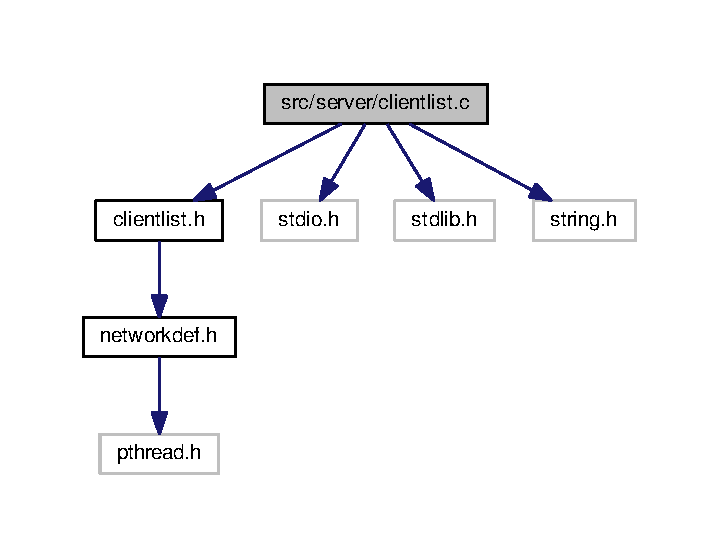
\includegraphics[width=345pt]{clientlist_8c__incl}
\end{center}
\end{figure}
\subsection*{Functions}
\begin{DoxyCompactItemize}
\item 
int \hyperlink{clientlist_8c_ada8804e2c519afb4f08a97e14c498b77}{compare} (struct \hyperlink{structClientInfo}{Client\+Info} $\ast$a, struct \hyperlink{structClientInfo}{Client\+Info} $\ast$b)
\begin{DoxyCompactList}\small\item\em Compare two {\ttfamily \hyperlink{structClientInfo}{Client\+Info}} struct, checking if they share the same connection socket. \end{DoxyCompactList}\item 
void \hyperlink{clientlist_8c_a0ab4922efddbeb22c4554a12301adfac}{list\+\_\+init} (struct \hyperlink{structLinkedList}{Linked\+List} $\ast$ll)
\begin{DoxyCompactList}\small\item\em Initialize an empty list. \end{DoxyCompactList}\item 
int \hyperlink{clientlist_8c_a6cea1cf625133bda1f22bd08c54659c0}{list\+\_\+insert} (struct \hyperlink{structLinkedList}{Linked\+List} $\ast$ll, struct \hyperlink{structClientInfo}{Client\+Info} $\ast$cl\+\_\+info)
\begin{DoxyCompactList}\small\item\em Insert a new element to the list. \end{DoxyCompactList}\item 
int \hyperlink{clientlist_8c_acb1d4dfa3cfe0c12c48bb6c237b88a24}{list\+\_\+delete} (struct \hyperlink{structLinkedList}{Linked\+List} $\ast$ll, struct \hyperlink{structClientInfo}{Client\+Info} $\ast$cl\+\_\+info)
\begin{DoxyCompactList}\small\item\em Delete a node from the list. \end{DoxyCompactList}\item 
void \hyperlink{clientlist_8c_a27550fe0a8fae43069d7fc80735ebfa3}{list\+\_\+dump} (struct \hyperlink{structLinkedList}{Linked\+List} $\ast$ll)
\begin{DoxyCompactList}\small\item\em Print the list in a readable format. \end{DoxyCompactList}\item 
int \hyperlink{clientlist_8c_a9b6ae95fc1c6a731fd23bc4976406bcc}{list\+\_\+size} (struct \hyperlink{structLinkedList}{Linked\+List} $\ast$ll)
\begin{DoxyCompactList}\small\item\em Returns the size of the linked list. \end{DoxyCompactList}\item 
char $\ast$$\ast$ \hyperlink{clientlist_8c_a849ee8fee1745818db7ab46b1770783b}{list\+\_\+clients} (struct \hyperlink{structLinkedList}{Linked\+List} $\ast$ll)
\begin{DoxyCompactList}\small\item\em Returns an array of strings containing the client\textquotesingle{}s aliases. \end{DoxyCompactList}\end{DoxyCompactItemize}


\subsection{Detailed Description}
Linked list implementation where every node represent a connection with a client. 

\begin{DoxyAuthor}{Author}
Enrico Vianello (\href{mailto:enrico.vianello.1@studenti.unipd.it}{\tt enrico.\+vianello.\+1@studenti.\+unipd.\+it}) 
\end{DoxyAuthor}
\begin{DoxyVersion}{Version}
1.\+0 
\end{DoxyVersion}
\begin{DoxySince}{Since}
1.\+0
\end{DoxySince}
\begin{DoxyCopyright}{Copyright}
Copyright (c) 2016-\/2017, Enrico Vianello 
\end{DoxyCopyright}


\subsection{Function Documentation}
\index{clientlist.\+c@{clientlist.\+c}!compare@{compare}}
\index{compare@{compare}!clientlist.\+c@{clientlist.\+c}}
\subsubsection[{\texorpdfstring{compare(struct Client\+Info $\ast$a, struct Client\+Info $\ast$b)}{compare(struct ClientInfo *a, struct ClientInfo *b)}}]{\setlength{\rightskip}{0pt plus 5cm}int compare (
\begin{DoxyParamCaption}
\item[{struct {\bf Client\+Info} $\ast$}]{a, }
\item[{struct {\bf Client\+Info} $\ast$}]{b}
\end{DoxyParamCaption}
)}\hypertarget{clientlist_8c_ada8804e2c519afb4f08a97e14c498b77}{}\label{clientlist_8c_ada8804e2c519afb4f08a97e14c498b77}


Compare two {\ttfamily \hyperlink{structClientInfo}{Client\+Info}} struct, checking if they share the same connection socket. 


\begin{DoxyParams}{Parameters}
{\em a} & Pointer to the first \hyperlink{structClientInfo}{Client\+Info} struct. \\
\hline
{\em b} & Pointer to the second \hyperlink{structClientInfo}{Client\+Info} struct.\\
\hline
\end{DoxyParams}
\begin{DoxyReturn}{Returns}
{\ttfamily 0} if they have the same connection socket. 
\end{DoxyReturn}
\index{clientlist.\+c@{clientlist.\+c}!list\+\_\+clients@{list\+\_\+clients}}
\index{list\+\_\+clients@{list\+\_\+clients}!clientlist.\+c@{clientlist.\+c}}
\subsubsection[{\texorpdfstring{list\+\_\+clients(struct Linked\+List $\ast$ll)}{list_clients(struct LinkedList *ll)}}]{\setlength{\rightskip}{0pt plus 5cm}char$\ast$$\ast$ list\+\_\+clients (
\begin{DoxyParamCaption}
\item[{struct {\bf Linked\+List} $\ast$}]{ll}
\end{DoxyParamCaption}
)}\hypertarget{clientlist_8c_a849ee8fee1745818db7ab46b1770783b}{}\label{clientlist_8c_a849ee8fee1745818db7ab46b1770783b}


Returns an array of strings containing the client\textquotesingle{}s aliases. 

This method allocate the memory necessary to store the list, so make sure to deallocate using the pointer returned.


\begin{DoxyParams}{Parameters}
{\em ll} & Pointer to the linked list.\\
\hline
\end{DoxyParams}
\begin{DoxyReturn}{Returns}
An array of strings containing the aliases field of the objects {\ttfamily \hyperlink{structClientInfo}{Client\+Info}} in the list. 
\end{DoxyReturn}
\index{clientlist.\+c@{clientlist.\+c}!list\+\_\+delete@{list\+\_\+delete}}
\index{list\+\_\+delete@{list\+\_\+delete}!clientlist.\+c@{clientlist.\+c}}
\subsubsection[{\texorpdfstring{list\+\_\+delete(struct Linked\+List $\ast$ll, struct Client\+Info $\ast$cl\+\_\+info)}{list_delete(struct LinkedList *ll, struct ClientInfo *cl_info)}}]{\setlength{\rightskip}{0pt plus 5cm}int list\+\_\+delete (
\begin{DoxyParamCaption}
\item[{struct {\bf Linked\+List} $\ast$}]{ll, }
\item[{struct {\bf Client\+Info} $\ast$}]{cl\+\_\+info}
\end{DoxyParamCaption}
)}\hypertarget{clientlist_8c_acb1d4dfa3cfe0c12c48bb6c237b88a24}{}\label{clientlist_8c_acb1d4dfa3cfe0c12c48bb6c237b88a24}


Delete a node from the list. 


\begin{DoxyParams}{Parameters}
{\em ll} & Pointer to the linked list. \\
\hline
{\em cl\+\_\+info} & Pointer to the {\ttfamily \hyperlink{structClientInfo}{Client\+Info}} structure of the node that has to be removed.\\
\hline
\end{DoxyParams}
\begin{DoxyReturn}{Returns}
{\ttfamily 0} if successful, {\ttfamily -\/1} if the list is empty or an error occours. 
\end{DoxyReturn}
\index{clientlist.\+c@{clientlist.\+c}!list\+\_\+dump@{list\+\_\+dump}}
\index{list\+\_\+dump@{list\+\_\+dump}!clientlist.\+c@{clientlist.\+c}}
\subsubsection[{\texorpdfstring{list\+\_\+dump(struct Linked\+List $\ast$ll)}{list_dump(struct LinkedList *ll)}}]{\setlength{\rightskip}{0pt plus 5cm}void list\+\_\+dump (
\begin{DoxyParamCaption}
\item[{struct {\bf Linked\+List} $\ast$}]{ll}
\end{DoxyParamCaption}
)}\hypertarget{clientlist_8c_a27550fe0a8fae43069d7fc80735ebfa3}{}\label{clientlist_8c_a27550fe0a8fae43069d7fc80735ebfa3}


Print the list in a readable format. 


\begin{DoxyParams}{Parameters}
{\em ll} & Pointer to the linked list. \\
\hline
\end{DoxyParams}
\index{clientlist.\+c@{clientlist.\+c}!list\+\_\+init@{list\+\_\+init}}
\index{list\+\_\+init@{list\+\_\+init}!clientlist.\+c@{clientlist.\+c}}
\subsubsection[{\texorpdfstring{list\+\_\+init(struct Linked\+List $\ast$ll)}{list_init(struct LinkedList *ll)}}]{\setlength{\rightskip}{0pt plus 5cm}void list\+\_\+init (
\begin{DoxyParamCaption}
\item[{struct {\bf Linked\+List} $\ast$}]{ll}
\end{DoxyParamCaption}
)}\hypertarget{clientlist_8c_a0ab4922efddbeb22c4554a12301adfac}{}\label{clientlist_8c_a0ab4922efddbeb22c4554a12301adfac}


Initialize an empty list. 


\begin{DoxyParams}{Parameters}
{\em ll} & Pointer to the linked list. \\
\hline
\end{DoxyParams}
\index{clientlist.\+c@{clientlist.\+c}!list\+\_\+insert@{list\+\_\+insert}}
\index{list\+\_\+insert@{list\+\_\+insert}!clientlist.\+c@{clientlist.\+c}}
\subsubsection[{\texorpdfstring{list\+\_\+insert(struct Linked\+List $\ast$ll, struct Client\+Info $\ast$cl\+\_\+info)}{list_insert(struct LinkedList *ll, struct ClientInfo *cl_info)}}]{\setlength{\rightskip}{0pt plus 5cm}int list\+\_\+insert (
\begin{DoxyParamCaption}
\item[{struct {\bf Linked\+List} $\ast$}]{ll, }
\item[{struct {\bf Client\+Info} $\ast$}]{cl\+\_\+info}
\end{DoxyParamCaption}
)}\hypertarget{clientlist_8c_a6cea1cf625133bda1f22bd08c54659c0}{}\label{clientlist_8c_a6cea1cf625133bda1f22bd08c54659c0}


Insert a new element to the list. 


\begin{DoxyParams}{Parameters}
{\em ll} & Pointer to the linked list. \\
\hline
{\em cl\+\_\+info} & Pointer to the {\ttfamily \hyperlink{structClientInfo}{Client\+Info}} structure that will be contained in the new node.\\
\hline
\end{DoxyParams}
\begin{DoxyReturn}{Returns}
{\ttfamily 0} if successful, {\ttfamily -\/1} if the list is full or an error occours. 
\end{DoxyReturn}
\index{clientlist.\+c@{clientlist.\+c}!list\+\_\+size@{list\+\_\+size}}
\index{list\+\_\+size@{list\+\_\+size}!clientlist.\+c@{clientlist.\+c}}
\subsubsection[{\texorpdfstring{list\+\_\+size(struct Linked\+List $\ast$ll)}{list_size(struct LinkedList *ll)}}]{\setlength{\rightskip}{0pt plus 5cm}int list\+\_\+size (
\begin{DoxyParamCaption}
\item[{struct {\bf Linked\+List} $\ast$}]{ll}
\end{DoxyParamCaption}
)}\hypertarget{clientlist_8c_a9b6ae95fc1c6a731fd23bc4976406bcc}{}\label{clientlist_8c_a9b6ae95fc1c6a731fd23bc4976406bcc}


Returns the size of the linked list. 


\begin{DoxyParams}{Parameters}
{\em ll} & Pointer to the linked list.\\
\hline
\end{DoxyParams}
\begin{DoxyReturn}{Returns}
An {\ttfamily int} representing the number of nodes in the list. 
\end{DoxyReturn}

\hypertarget{clientlist_8h}{}\section{src/server/clientlist.h File Reference}
\label{clientlist_8h}\index{src/server/clientlist.\+h@{src/server/clientlist.\+h}}


Linked list implementation where every node represent a connection with a client.  


{\ttfamily \#include \char`\"{}networkdef.\+h\char`\"{}}\\*
Include dependency graph for clientlist.\+h\+:\nopagebreak
\begin{figure}[H]
\begin{center}
\leavevmode
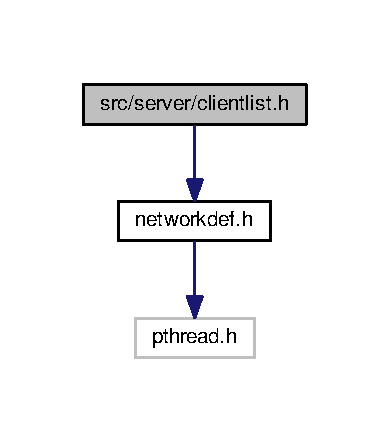
\includegraphics[width=187pt]{clientlist_8h__incl}
\end{center}
\end{figure}
This graph shows which files directly or indirectly include this file\+:\nopagebreak
\begin{figure}[H]
\begin{center}
\leavevmode
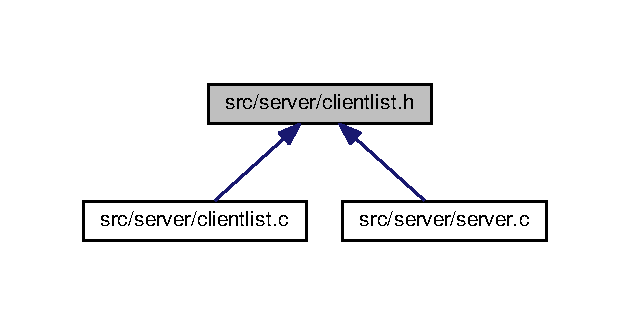
\includegraphics[width=303pt]{clientlist_8h__dep__incl}
\end{center}
\end{figure}
\subsection*{Data Structures}
\begin{DoxyCompactItemize}
\item 
struct \hyperlink{structLLNode}{L\+L\+Node}
\begin{DoxyCompactList}\small\item\em Node of the linked list, representing a connection. \end{DoxyCompactList}\item 
struct \hyperlink{structLinkedList}{Linked\+List}
\begin{DoxyCompactList}\small\item\em Linked list structure. \end{DoxyCompactList}\end{DoxyCompactItemize}
\subsection*{Functions}
\begin{DoxyCompactItemize}
\item 
int \hyperlink{clientlist_8h_ada8804e2c519afb4f08a97e14c498b77}{compare} (struct \hyperlink{structClientInfo}{Client\+Info} $\ast$a, struct \hyperlink{structClientInfo}{Client\+Info} $\ast$b)
\begin{DoxyCompactList}\small\item\em Compare two {\ttfamily \hyperlink{structClientInfo}{Client\+Info}} struct, checking if they share the same connection socket. \end{DoxyCompactList}\item 
void \hyperlink{clientlist_8h_a0ab4922efddbeb22c4554a12301adfac}{list\+\_\+init} (struct \hyperlink{structLinkedList}{Linked\+List} $\ast$ll)
\begin{DoxyCompactList}\small\item\em Initialize an empty list. \end{DoxyCompactList}\item 
int \hyperlink{clientlist_8h_a6cea1cf625133bda1f22bd08c54659c0}{list\+\_\+insert} (struct \hyperlink{structLinkedList}{Linked\+List} $\ast$ll, struct \hyperlink{structClientInfo}{Client\+Info} $\ast$cl\+\_\+info)
\begin{DoxyCompactList}\small\item\em Insert a new element to the list. \end{DoxyCompactList}\item 
int \hyperlink{clientlist_8h_acb1d4dfa3cfe0c12c48bb6c237b88a24}{list\+\_\+delete} (struct \hyperlink{structLinkedList}{Linked\+List} $\ast$ll, struct \hyperlink{structClientInfo}{Client\+Info} $\ast$cl\+\_\+info)
\begin{DoxyCompactList}\small\item\em Delete a node from the list. \end{DoxyCompactList}\item 
void \hyperlink{clientlist_8h_a27550fe0a8fae43069d7fc80735ebfa3}{list\+\_\+dump} (struct \hyperlink{structLinkedList}{Linked\+List} $\ast$ll)
\begin{DoxyCompactList}\small\item\em Print the list in a readable format. \end{DoxyCompactList}\item 
int \hyperlink{clientlist_8h_a9b6ae95fc1c6a731fd23bc4976406bcc}{list\+\_\+size} (struct \hyperlink{structLinkedList}{Linked\+List} $\ast$ll)
\begin{DoxyCompactList}\small\item\em Returns the size of the linked list. \end{DoxyCompactList}\item 
char $\ast$$\ast$ \hyperlink{clientlist_8h_a849ee8fee1745818db7ab46b1770783b}{list\+\_\+clients} (struct \hyperlink{structLinkedList}{Linked\+List} $\ast$ll)
\begin{DoxyCompactList}\small\item\em Returns an array of strings containing the client\textquotesingle{}s aliases. \end{DoxyCompactList}\end{DoxyCompactItemize}


\subsection{Detailed Description}
Linked list implementation where every node represent a connection with a client. 

\begin{DoxyAuthor}{Author}
Enrico Vianello (\href{mailto:enrico.vianello.1@studenti.unipd.it}{\tt enrico.\+vianello.\+1@studenti.\+unipd.\+it}) 
\end{DoxyAuthor}
\begin{DoxyVersion}{Version}
1.\+0 
\end{DoxyVersion}
\begin{DoxySince}{Since}
1.\+0
\end{DoxySince}
\begin{DoxyCopyright}{Copyright}
Copyright (c) 2016-\/2017, Enrico Vianello 
\end{DoxyCopyright}


\subsection{Function Documentation}
\index{clientlist.\+h@{clientlist.\+h}!compare@{compare}}
\index{compare@{compare}!clientlist.\+h@{clientlist.\+h}}
\subsubsection[{\texorpdfstring{compare(struct Client\+Info $\ast$a, struct Client\+Info $\ast$b)}{compare(struct ClientInfo *a, struct ClientInfo *b)}}]{\setlength{\rightskip}{0pt plus 5cm}int compare (
\begin{DoxyParamCaption}
\item[{struct {\bf Client\+Info} $\ast$}]{a, }
\item[{struct {\bf Client\+Info} $\ast$}]{b}
\end{DoxyParamCaption}
)}\hypertarget{clientlist_8h_ada8804e2c519afb4f08a97e14c498b77}{}\label{clientlist_8h_ada8804e2c519afb4f08a97e14c498b77}


Compare two {\ttfamily \hyperlink{structClientInfo}{Client\+Info}} struct, checking if they share the same connection socket. 


\begin{DoxyParams}{Parameters}
{\em a} & Pointer to the first \hyperlink{structClientInfo}{Client\+Info} struct. \\
\hline
{\em b} & Pointer to the second \hyperlink{structClientInfo}{Client\+Info} struct.\\
\hline
\end{DoxyParams}
\begin{DoxyReturn}{Returns}
{\ttfamily 0} if they have the same connection socket. 
\end{DoxyReturn}
\index{clientlist.\+h@{clientlist.\+h}!list\+\_\+clients@{list\+\_\+clients}}
\index{list\+\_\+clients@{list\+\_\+clients}!clientlist.\+h@{clientlist.\+h}}
\subsubsection[{\texorpdfstring{list\+\_\+clients(struct Linked\+List $\ast$ll)}{list_clients(struct LinkedList *ll)}}]{\setlength{\rightskip}{0pt plus 5cm}char$\ast$$\ast$ list\+\_\+clients (
\begin{DoxyParamCaption}
\item[{struct {\bf Linked\+List} $\ast$}]{ll}
\end{DoxyParamCaption}
)}\hypertarget{clientlist_8h_a849ee8fee1745818db7ab46b1770783b}{}\label{clientlist_8h_a849ee8fee1745818db7ab46b1770783b}


Returns an array of strings containing the client\textquotesingle{}s aliases. 

This method allocate the memory necessary to store the list, so make sure to deallocate using the pointer returned.


\begin{DoxyParams}{Parameters}
{\em ll} & Pointer to the linked list.\\
\hline
\end{DoxyParams}
\begin{DoxyReturn}{Returns}
An array of strings containing the aliases field of the objects {\ttfamily \hyperlink{structClientInfo}{Client\+Info}} in the list. 
\end{DoxyReturn}
\index{clientlist.\+h@{clientlist.\+h}!list\+\_\+delete@{list\+\_\+delete}}
\index{list\+\_\+delete@{list\+\_\+delete}!clientlist.\+h@{clientlist.\+h}}
\subsubsection[{\texorpdfstring{list\+\_\+delete(struct Linked\+List $\ast$ll, struct Client\+Info $\ast$cl\+\_\+info)}{list_delete(struct LinkedList *ll, struct ClientInfo *cl_info)}}]{\setlength{\rightskip}{0pt plus 5cm}int list\+\_\+delete (
\begin{DoxyParamCaption}
\item[{struct {\bf Linked\+List} $\ast$}]{ll, }
\item[{struct {\bf Client\+Info} $\ast$}]{cl\+\_\+info}
\end{DoxyParamCaption}
)}\hypertarget{clientlist_8h_acb1d4dfa3cfe0c12c48bb6c237b88a24}{}\label{clientlist_8h_acb1d4dfa3cfe0c12c48bb6c237b88a24}


Delete a node from the list. 


\begin{DoxyParams}{Parameters}
{\em ll} & Pointer to the linked list. \\
\hline
{\em cl\+\_\+info} & Pointer to the {\ttfamily \hyperlink{structClientInfo}{Client\+Info}} structure of the node that has to be removed.\\
\hline
\end{DoxyParams}
\begin{DoxyReturn}{Returns}
{\ttfamily 0} if successful, {\ttfamily -\/1} if the list is empty or an error occours. 
\end{DoxyReturn}
\index{clientlist.\+h@{clientlist.\+h}!list\+\_\+dump@{list\+\_\+dump}}
\index{list\+\_\+dump@{list\+\_\+dump}!clientlist.\+h@{clientlist.\+h}}
\subsubsection[{\texorpdfstring{list\+\_\+dump(struct Linked\+List $\ast$ll)}{list_dump(struct LinkedList *ll)}}]{\setlength{\rightskip}{0pt plus 5cm}void list\+\_\+dump (
\begin{DoxyParamCaption}
\item[{struct {\bf Linked\+List} $\ast$}]{ll}
\end{DoxyParamCaption}
)}\hypertarget{clientlist_8h_a27550fe0a8fae43069d7fc80735ebfa3}{}\label{clientlist_8h_a27550fe0a8fae43069d7fc80735ebfa3}


Print the list in a readable format. 


\begin{DoxyParams}{Parameters}
{\em ll} & Pointer to the linked list. \\
\hline
\end{DoxyParams}
\index{clientlist.\+h@{clientlist.\+h}!list\+\_\+init@{list\+\_\+init}}
\index{list\+\_\+init@{list\+\_\+init}!clientlist.\+h@{clientlist.\+h}}
\subsubsection[{\texorpdfstring{list\+\_\+init(struct Linked\+List $\ast$ll)}{list_init(struct LinkedList *ll)}}]{\setlength{\rightskip}{0pt plus 5cm}void list\+\_\+init (
\begin{DoxyParamCaption}
\item[{struct {\bf Linked\+List} $\ast$}]{ll}
\end{DoxyParamCaption}
)}\hypertarget{clientlist_8h_a0ab4922efddbeb22c4554a12301adfac}{}\label{clientlist_8h_a0ab4922efddbeb22c4554a12301adfac}


Initialize an empty list. 


\begin{DoxyParams}{Parameters}
{\em ll} & Pointer to the linked list. \\
\hline
\end{DoxyParams}
\index{clientlist.\+h@{clientlist.\+h}!list\+\_\+insert@{list\+\_\+insert}}
\index{list\+\_\+insert@{list\+\_\+insert}!clientlist.\+h@{clientlist.\+h}}
\subsubsection[{\texorpdfstring{list\+\_\+insert(struct Linked\+List $\ast$ll, struct Client\+Info $\ast$cl\+\_\+info)}{list_insert(struct LinkedList *ll, struct ClientInfo *cl_info)}}]{\setlength{\rightskip}{0pt plus 5cm}int list\+\_\+insert (
\begin{DoxyParamCaption}
\item[{struct {\bf Linked\+List} $\ast$}]{ll, }
\item[{struct {\bf Client\+Info} $\ast$}]{cl\+\_\+info}
\end{DoxyParamCaption}
)}\hypertarget{clientlist_8h_a6cea1cf625133bda1f22bd08c54659c0}{}\label{clientlist_8h_a6cea1cf625133bda1f22bd08c54659c0}


Insert a new element to the list. 


\begin{DoxyParams}{Parameters}
{\em ll} & Pointer to the linked list. \\
\hline
{\em cl\+\_\+info} & Pointer to the {\ttfamily \hyperlink{structClientInfo}{Client\+Info}} structure that will be contained in the new node.\\
\hline
\end{DoxyParams}
\begin{DoxyReturn}{Returns}
{\ttfamily 0} if successful, {\ttfamily -\/1} if the list is full or an error occours. 
\end{DoxyReturn}
\index{clientlist.\+h@{clientlist.\+h}!list\+\_\+size@{list\+\_\+size}}
\index{list\+\_\+size@{list\+\_\+size}!clientlist.\+h@{clientlist.\+h}}
\subsubsection[{\texorpdfstring{list\+\_\+size(struct Linked\+List $\ast$ll)}{list_size(struct LinkedList *ll)}}]{\setlength{\rightskip}{0pt plus 5cm}int list\+\_\+size (
\begin{DoxyParamCaption}
\item[{struct {\bf Linked\+List} $\ast$}]{ll}
\end{DoxyParamCaption}
)}\hypertarget{clientlist_8h_a9b6ae95fc1c6a731fd23bc4976406bcc}{}\label{clientlist_8h_a9b6ae95fc1c6a731fd23bc4976406bcc}


Returns the size of the linked list. 


\begin{DoxyParams}{Parameters}
{\em ll} & Pointer to the linked list.\\
\hline
\end{DoxyParams}
\begin{DoxyReturn}{Returns}
An {\ttfamily int} representing the number of nodes in the list. 
\end{DoxyReturn}

\hypertarget{server_8c}{}\section{src/server/server.c File Reference}
\label{server_8c}\index{src/server/server.\+c@{src/server/server.\+c}}


Server chat application for the c-\/chat project.  


{\ttfamily \#include \char`\"{}server.\+h\char`\"{}}\\*
{\ttfamily \#include \char`\"{}networkutil.\+h\char`\"{}}\\*
{\ttfamily \#include \char`\"{}clientlist.\+h\char`\"{}}\\*
{\ttfamily \#include $<$stdio.\+h$>$}\\*
{\ttfamily \#include $<$stdlib.\+h$>$}\\*
{\ttfamily \#include $<$unistd.\+h$>$}\\*
{\ttfamily \#include $<$errno.\+h$>$}\\*
{\ttfamily \#include $<$string.\+h$>$}\\*
{\ttfamily \#include $<$stdint.\+h$>$}\\*
{\ttfamily \#include $<$sys/types.\+h$>$}\\*
{\ttfamily \#include $<$sys/socket.\+h$>$}\\*
{\ttfamily \#include $<$netinet/in.\+h$>$}\\*
{\ttfamily \#include $<$netdb.\+h$>$}\\*
{\ttfamily \#include $<$arpa/inet.\+h$>$}\\*
{\ttfamily \#include $<$sys/wait.\+h$>$}\\*
{\ttfamily \#include $<$signal.\+h$>$}\\*
{\ttfamily \#include $<$pthread.\+h$>$}\\*
Include dependency graph for server.\+c\+:\nopagebreak
\begin{figure}[H]
\begin{center}
\leavevmode
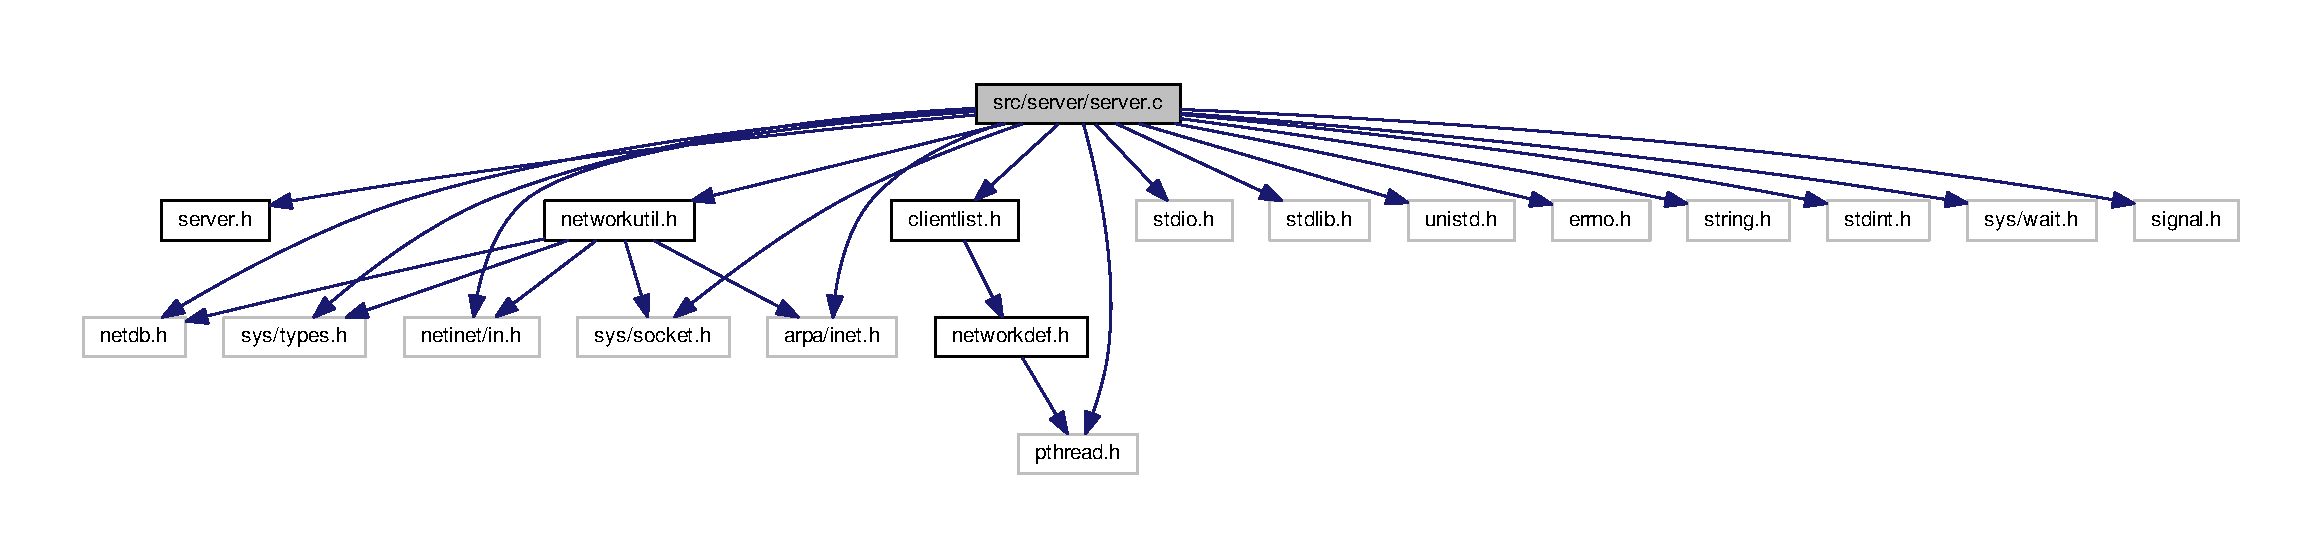
\includegraphics[width=350pt]{server_8c__incl}
\end{center}
\end{figure}
\subsection*{Functions}
\begin{DoxyCompactItemize}
\item 
int \hyperlink{server_8c_a212d06967c429e15dd341c0dd0458336}{displayhelp} ()
\begin{DoxyCompactList}\small\item\em Display the available commands. \end{DoxyCompactList}\item 
void $\ast$ \hyperlink{server_8c_ae4e2cf910fd8d0299a5b8af57b227e1a}{server\+\_\+handler} (void $\ast$param)
\begin{DoxyCompactList}\small\item\em Routine that listens for server\textquotesingle{}s commands. \end{DoxyCompactList}\item 
void $\ast$ \hyperlink{server_8c_a01cae930ab07840bbe7d320b62c2e8cb}{client\+\_\+handler} (void $\ast$info)
\begin{DoxyCompactList}\small\item\em Routine that handles the connection with a client. \end{DoxyCompactList}\item 
int {\bfseries main} (int argc, char $\ast$argv\mbox{[}$\,$\mbox{]})\hypertarget{server_8c_a0ddf1224851353fc92bfbff6f499fa97}{}\label{server_8c_a0ddf1224851353fc92bfbff6f499fa97}

\end{DoxyCompactItemize}
\subsection*{Variables}
\begin{DoxyCompactItemize}
\item 
int \hyperlink{server_8c_a25061bc9654fbfab5356e6325daeab1d}{connectfd}
\item 
struct addrinfo \hyperlink{server_8c_ae56688bf50625537b553b45a9b68b808}{hints}
\item 
struct addrinfo $\ast$ \hyperlink{server_8c_aef3b9e5534e034ca3f4476a49a3e3105}{servinfo}
\item 
struct \hyperlink{structLinkedList}{Linked\+List} \hyperlink{server_8c_a6697f11f67991566ab4d0197cd78bf9f}{client\+\_\+list}
\item 
pthread\+\_\+mutex\+\_\+t \hyperlink{server_8c_a1cc31a41b454569942e2988ea151a7e5}{clientlist\+\_\+mutex}
\end{DoxyCompactItemize}


\subsection{Detailed Description}
Server chat application for the c-\/chat project. 

\begin{DoxyAuthor}{Author}
Enrico Vianello (\href{mailto:enrico.vianello.1@studenti.unipd.it}{\tt enrico.\+vianello.\+1@studenti.\+unipd.\+it}) 
\end{DoxyAuthor}
\begin{DoxyVersion}{Version}
1.\+0 
\end{DoxyVersion}
\begin{DoxySince}{Since}
1.\+0
\end{DoxySince}
\begin{DoxyCopyright}{Copyright}
Copyright (c) 2016-\/2017, Enrico Vianello 
\end{DoxyCopyright}


\subsection{Function Documentation}
\index{server.\+c@{server.\+c}!client\+\_\+handler@{client\+\_\+handler}}
\index{client\+\_\+handler@{client\+\_\+handler}!server.\+c@{server.\+c}}
\subsubsection[{\texorpdfstring{client\+\_\+handler(void $\ast$info)}{client_handler(void *info)}}]{\setlength{\rightskip}{0pt plus 5cm}void $\ast$ client\+\_\+handler (
\begin{DoxyParamCaption}
\item[{void $\ast$}]{info}
\end{DoxyParamCaption}
)}\hypertarget{server_8c_a01cae930ab07840bbe7d320b62c2e8cb}{}\label{server_8c_a01cae930ab07840bbe7d320b62c2e8cb}


Routine that handles the connection with a client. 


\begin{DoxyParams}{Parameters}
{\em info} & Pointer to the {\ttfamily \hyperlink{structClientInfo}{Client\+Info}} structure relative to the connection that has to be handled.\\
\hline
\end{DoxyParams}
\begin{DoxyReturn}{Returns}
Always a {\ttfamily N\+U\+LL} pointer. 
\end{DoxyReturn}
\index{server.\+c@{server.\+c}!displayhelp@{displayhelp}}
\index{displayhelp@{displayhelp}!server.\+c@{server.\+c}}
\subsubsection[{\texorpdfstring{displayhelp()}{displayhelp()}}]{\setlength{\rightskip}{0pt plus 5cm}int displayhelp (
\begin{DoxyParamCaption}
{}
\end{DoxyParamCaption}
)}\hypertarget{server_8c_a212d06967c429e15dd341c0dd0458336}{}\label{server_8c_a212d06967c429e15dd341c0dd0458336}


Display the available commands. 

\begin{DoxyReturn}{Returns}
{\ttfamily 0} if successful, {\ttfamily -\/1} if an error occurred. 
\end{DoxyReturn}
\index{server.\+c@{server.\+c}!server\+\_\+handler@{server\+\_\+handler}}
\index{server\+\_\+handler@{server\+\_\+handler}!server.\+c@{server.\+c}}
\subsubsection[{\texorpdfstring{server\+\_\+handler(void $\ast$param)}{server_handler(void *param)}}]{\setlength{\rightskip}{0pt plus 5cm}void $\ast$ server\+\_\+handler (
\begin{DoxyParamCaption}
\item[{void $\ast$}]{param}
\end{DoxyParamCaption}
)}\hypertarget{server_8c_ae4e2cf910fd8d0299a5b8af57b227e1a}{}\label{server_8c_ae4e2cf910fd8d0299a5b8af57b227e1a}


Routine that listens for server\textquotesingle{}s commands. 


\begin{DoxyParams}{Parameters}
{\em param} & Pointer to a structure containing execution parameters (currently unused, it can be safely set as {\ttfamily N\+U\+LL} pointer).\\
\hline
\end{DoxyParams}
\begin{DoxyReturn}{Returns}
Always a {\ttfamily N\+U\+LL} pointer. 
\end{DoxyReturn}


\subsection{Variable Documentation}
\index{server.\+c@{server.\+c}!client\+\_\+list@{client\+\_\+list}}
\index{client\+\_\+list@{client\+\_\+list}!server.\+c@{server.\+c}}
\subsubsection[{\texorpdfstring{client\+\_\+list}{client_list}}]{\setlength{\rightskip}{0pt plus 5cm}struct {\bf Linked\+List} client\+\_\+list}\hypertarget{server_8c_a6697f11f67991566ab4d0197cd78bf9f}{}\label{server_8c_a6697f11f67991566ab4d0197cd78bf9f}
List of the connected clients. \index{server.\+c@{server.\+c}!clientlist\+\_\+mutex@{clientlist\+\_\+mutex}}
\index{clientlist\+\_\+mutex@{clientlist\+\_\+mutex}!server.\+c@{server.\+c}}
\subsubsection[{\texorpdfstring{clientlist\+\_\+mutex}{clientlist_mutex}}]{\setlength{\rightskip}{0pt plus 5cm}pthread\+\_\+mutex\+\_\+t clientlist\+\_\+mutex}\hypertarget{server_8c_a1cc31a41b454569942e2988ea151a7e5}{}\label{server_8c_a1cc31a41b454569942e2988ea151a7e5}
Mutual exclusion variable preventing concurrent edits to the client list. \index{server.\+c@{server.\+c}!connectfd@{connectfd}}
\index{connectfd@{connectfd}!server.\+c@{server.\+c}}
\subsubsection[{\texorpdfstring{connectfd}{connectfd}}]{\setlength{\rightskip}{0pt plus 5cm}int connectfd}\hypertarget{server_8c_a25061bc9654fbfab5356e6325daeab1d}{}\label{server_8c_a25061bc9654fbfab5356e6325daeab1d}
Socket to perform actions. \index{server.\+c@{server.\+c}!hints@{hints}}
\index{hints@{hints}!server.\+c@{server.\+c}}
\subsubsection[{\texorpdfstring{hints}{hints}}]{\setlength{\rightskip}{0pt plus 5cm}struct addrinfo hints}\hypertarget{server_8c_ae56688bf50625537b553b45a9b68b808}{}\label{server_8c_ae56688bf50625537b553b45a9b68b808}
Structure used to set the preferencies for servinfo. \index{server.\+c@{server.\+c}!servinfo@{servinfo}}
\index{servinfo@{servinfo}!server.\+c@{server.\+c}}
\subsubsection[{\texorpdfstring{servinfo}{servinfo}}]{\setlength{\rightskip}{0pt plus 5cm}struct addrinfo$\ast$ servinfo}\hypertarget{server_8c_aef3b9e5534e034ca3f4476a49a3e3105}{}\label{server_8c_aef3b9e5534e034ca3f4476a49a3e3105}
Structure containing local data. 
\hypertarget{server_8h}{}\section{src/server/server.h File Reference}
\label{server_8h}\index{src/server/server.\+h@{src/server/server.\+h}}


Server chat application for the c-\/chat project.  


This graph shows which files directly or indirectly include this file\+:\nopagebreak
\begin{figure}[H]
\begin{center}
\leavevmode
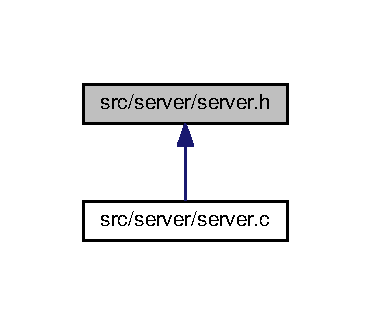
\includegraphics[width=178pt]{server_8h__dep__incl}
\end{center}
\end{figure}
\subsection*{Macros}
\begin{DoxyCompactItemize}
\item 
\#define \hyperlink{server_8h_a826f1ffd868d8028516cdb7e80919825}{S\+E\+R\+V\+E\+R\+IP}~\char`\"{}localhost\char`\"{}
\item 
\#define \hyperlink{server_8h_a82cd61d8dfabc6a7d9ab209995f85e93}{S\+E\+R\+V\+E\+R\+P\+O\+RT}~\char`\"{}3495\char`\"{}
\item 
\#define \hyperlink{server_8h_aeefbbafa97642defe3ee6c3080b7d66f}{B\+A\+C\+K\+L\+OG}~8
\end{DoxyCompactItemize}


\subsection{Detailed Description}
Server chat application for the c-\/chat project. 

\begin{DoxyAuthor}{Author}
Enrico Vianello (\href{mailto:enrico.vianello.1@studenti.unipd.it}{\tt enrico.\+vianello.\+1@studenti.\+unipd.\+it}) 
\end{DoxyAuthor}
\begin{DoxyVersion}{Version}
1.\+0 
\end{DoxyVersion}
\begin{DoxySince}{Since}
1.\+0
\end{DoxySince}
\begin{DoxyCopyright}{Copyright}
Copyright (c) 2016-\/2017, Enrico Vianello 
\end{DoxyCopyright}


\subsection{Macro Definition Documentation}
\index{server.\+h@{server.\+h}!B\+A\+C\+K\+L\+OG@{B\+A\+C\+K\+L\+OG}}
\index{B\+A\+C\+K\+L\+OG@{B\+A\+C\+K\+L\+OG}!server.\+h@{server.\+h}}
\subsubsection[{\texorpdfstring{B\+A\+C\+K\+L\+OG}{BACKLOG}}]{\setlength{\rightskip}{0pt plus 5cm}\#define B\+A\+C\+K\+L\+OG~8}\hypertarget{server_8h_aeefbbafa97642defe3ee6c3080b7d66f}{}\label{server_8h_aeefbbafa97642defe3ee6c3080b7d66f}
How many pending connections queue will hold \index{server.\+h@{server.\+h}!S\+E\+R\+V\+E\+R\+IP@{S\+E\+R\+V\+E\+R\+IP}}
\index{S\+E\+R\+V\+E\+R\+IP@{S\+E\+R\+V\+E\+R\+IP}!server.\+h@{server.\+h}}
\subsubsection[{\texorpdfstring{S\+E\+R\+V\+E\+R\+IP}{SERVERIP}}]{\setlength{\rightskip}{0pt plus 5cm}\#define S\+E\+R\+V\+E\+R\+IP~\char`\"{}localhost\char`\"{}}\hypertarget{server_8h_a826f1ffd868d8028516cdb7e80919825}{}\label{server_8h_a826f1ffd868d8028516cdb7e80919825}
The server\textquotesingle{}s address \index{server.\+h@{server.\+h}!S\+E\+R\+V\+E\+R\+P\+O\+RT@{S\+E\+R\+V\+E\+R\+P\+O\+RT}}
\index{S\+E\+R\+V\+E\+R\+P\+O\+RT@{S\+E\+R\+V\+E\+R\+P\+O\+RT}!server.\+h@{server.\+h}}
\subsubsection[{\texorpdfstring{S\+E\+R\+V\+E\+R\+P\+O\+RT}{SERVERPORT}}]{\setlength{\rightskip}{0pt plus 5cm}\#define S\+E\+R\+V\+E\+R\+P\+O\+RT~\char`\"{}3495\char`\"{}}\hypertarget{server_8h_a82cd61d8dfabc6a7d9ab209995f85e93}{}\label{server_8h_a82cd61d8dfabc6a7d9ab209995f85e93}
Port used by the server for incoming connections 
\hypertarget{networkdef_8h}{}\section{src/util/networkdef.h File Reference}
\label{networkdef_8h}\index{src/util/networkdef.\+h@{src/util/networkdef.\+h}}


Parameters, structures and definitions relative to the applications\textquotesingle{} behaviour and the connection\textquotesingle{}s protocol.  


{\ttfamily \#include $<$pthread.\+h$>$}\\*
Include dependency graph for networkdef.\+h\+:\nopagebreak
\begin{figure}[H]
\begin{center}
\leavevmode
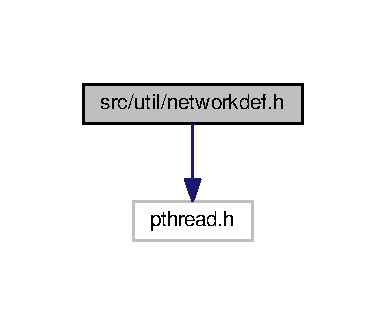
\includegraphics[width=185pt]{networkdef_8h__incl}
\end{center}
\end{figure}
This graph shows which files directly or indirectly include this file\+:\nopagebreak
\begin{figure}[H]
\begin{center}
\leavevmode
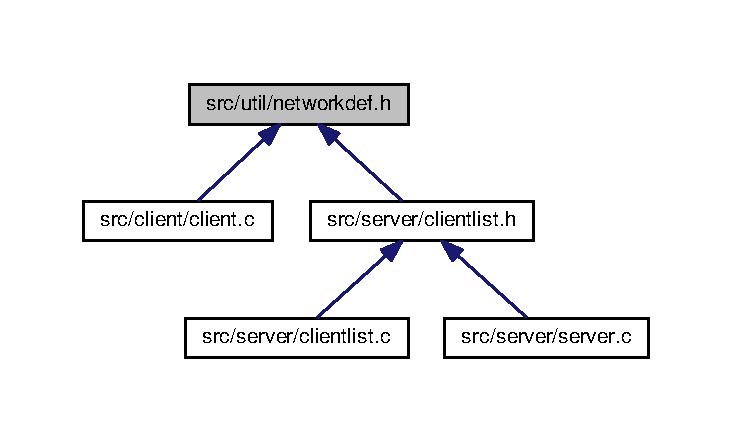
\includegraphics[width=350pt]{networkdef_8h__dep__incl}
\end{center}
\end{figure}
\subsection*{Data Structures}
\begin{DoxyCompactItemize}
\item 
struct \hyperlink{structClientInfo}{Client\+Info}
\begin{DoxyCompactList}\small\item\em Structure containing the informations regarding a single connection with a client. \end{DoxyCompactList}\item 
struct \hyperlink{structPacket}{Packet}
\begin{DoxyCompactList}\small\item\em Structure representing a single packet exchanged between the server and the clients. \end{DoxyCompactList}\end{DoxyCompactItemize}
\subsection*{Macros}
\begin{DoxyCompactItemize}
\item 
\#define \hyperlink{networkdef_8h_aa07ba58ae52cf11992b7e112454a3eea}{A\+L\+I\+A\+S\+L\+EN}~32
\item 
\#define \hyperlink{networkdef_8h_af83ab94da573d95ddc366030c5537d60}{C\+M\+D\+L\+EN}~32
\item 
\#define \hyperlink{networkdef_8h_aa8ece57a8603af32c591885469eb3b53}{D\+E\+F\+A\+U\+L\+T\+A\+L\+I\+AS}~\char`\"{}Anonymous\char`\"{}
\item 
\#define \hyperlink{networkdef_8h_a2ec728de0089ed37af934ae60ed1cd7f}{P\+A\+Y\+L\+EN}~2048
\item 
\#define \hyperlink{networkdef_8h_ace5c08f66edfc6ae44edaeef6b6101b6}{M\+A\+X\+C\+L\+I\+E\+N\+TS}~64
\item 
\#define \hyperlink{networkdef_8h_ad111e603bbebe5d87f6bc39264ce4733}{E\+X\+IT}~0
\item 
\#define \hyperlink{networkdef_8h_adf9402a5feb214522faa2cacb0a27403}{A\+L\+I\+AS}~1
\item 
\#define \hyperlink{networkdef_8h_a0c719c414608ef14852670b063876c07}{M\+SG}~2
\item 
\#define \hyperlink{networkdef_8h_a058161b004cade9fa3185c76022d92ed}{W\+H\+I\+S\+P\+ER}~3
\item 
\#define \hyperlink{networkdef_8h_a109c1cb0257bd1325c46dce538d5ec49}{S\+H\+O\+UT}~4
\item 
\#define \hyperlink{networkdef_8h_a035c351dbfe2787a071986245c7d2c57}{L\+I\+S\+T\+\_\+Q}~5
\item 
\#define \hyperlink{networkdef_8h_a36c0d2925720ebecbaf3469ff40fc6f8}{L\+I\+S\+T\+\_\+A}~6
\item 
\#define \hyperlink{networkdef_8h_a44ac67e8098ae79effe3d2abd710ad0e}{U\+NF}~7
\end{DoxyCompactItemize}


\subsection{Detailed Description}
Parameters, structures and definitions relative to the applications\textquotesingle{} behaviour and the connection\textquotesingle{}s protocol. 

\begin{DoxyAuthor}{Author}
Enrico Vianello (\href{mailto:enrico.vianello.1@studenti.unipd.it}{\tt enrico.\+vianello.\+1@studenti.\+unipd.\+it}) 
\end{DoxyAuthor}
\begin{DoxyVersion}{Version}
1.\+0 
\end{DoxyVersion}
\begin{DoxySince}{Since}
1.\+0
\end{DoxySince}
\begin{DoxyCopyright}{Copyright}
Copyright (c) 2016-\/2017, Enrico Vianello 
\end{DoxyCopyright}


\subsection{Macro Definition Documentation}
\index{networkdef.\+h@{networkdef.\+h}!A\+L\+I\+AS@{A\+L\+I\+AS}}
\index{A\+L\+I\+AS@{A\+L\+I\+AS}!networkdef.\+h@{networkdef.\+h}}
\subsubsection[{\texorpdfstring{A\+L\+I\+AS}{ALIAS}}]{\setlength{\rightskip}{0pt plus 5cm}\#define A\+L\+I\+AS~1}\hypertarget{networkdef_8h_adf9402a5feb214522faa2cacb0a27403}{}\label{networkdef_8h_adf9402a5feb214522faa2cacb0a27403}
alias changing request \index{networkdef.\+h@{networkdef.\+h}!A\+L\+I\+A\+S\+L\+EN@{A\+L\+I\+A\+S\+L\+EN}}
\index{A\+L\+I\+A\+S\+L\+EN@{A\+L\+I\+A\+S\+L\+EN}!networkdef.\+h@{networkdef.\+h}}
\subsubsection[{\texorpdfstring{A\+L\+I\+A\+S\+L\+EN}{ALIASLEN}}]{\setlength{\rightskip}{0pt plus 5cm}\#define A\+L\+I\+A\+S\+L\+EN~32}\hypertarget{networkdef_8h_aa07ba58ae52cf11992b7e112454a3eea}{}\label{networkdef_8h_aa07ba58ae52cf11992b7e112454a3eea}
Maximum length of the client\textquotesingle{}s aliases \index{networkdef.\+h@{networkdef.\+h}!C\+M\+D\+L\+EN@{C\+M\+D\+L\+EN}}
\index{C\+M\+D\+L\+EN@{C\+M\+D\+L\+EN}!networkdef.\+h@{networkdef.\+h}}
\subsubsection[{\texorpdfstring{C\+M\+D\+L\+EN}{CMDLEN}}]{\setlength{\rightskip}{0pt plus 5cm}\#define C\+M\+D\+L\+EN~32}\hypertarget{networkdef_8h_af83ab94da573d95ddc366030c5537d60}{}\label{networkdef_8h_af83ab94da573d95ddc366030c5537d60}
Maximum length of server\textquotesingle{}s and client\textquotesingle{}s commands \index{networkdef.\+h@{networkdef.\+h}!D\+E\+F\+A\+U\+L\+T\+A\+L\+I\+AS@{D\+E\+F\+A\+U\+L\+T\+A\+L\+I\+AS}}
\index{D\+E\+F\+A\+U\+L\+T\+A\+L\+I\+AS@{D\+E\+F\+A\+U\+L\+T\+A\+L\+I\+AS}!networkdef.\+h@{networkdef.\+h}}
\subsubsection[{\texorpdfstring{D\+E\+F\+A\+U\+L\+T\+A\+L\+I\+AS}{DEFAULTALIAS}}]{\setlength{\rightskip}{0pt plus 5cm}\#define D\+E\+F\+A\+U\+L\+T\+A\+L\+I\+AS~\char`\"{}Anonymous\char`\"{}}\hypertarget{networkdef_8h_aa8ece57a8603af32c591885469eb3b53}{}\label{networkdef_8h_aa8ece57a8603af32c591885469eb3b53}
Default alias for new clients \index{networkdef.\+h@{networkdef.\+h}!E\+X\+IT@{E\+X\+IT}}
\index{E\+X\+IT@{E\+X\+IT}!networkdef.\+h@{networkdef.\+h}}
\subsubsection[{\texorpdfstring{E\+X\+IT}{EXIT}}]{\setlength{\rightskip}{0pt plus 5cm}\#define E\+X\+IT~0}\hypertarget{networkdef_8h_ad111e603bbebe5d87f6bc39264ce4733}{}\label{networkdef_8h_ad111e603bbebe5d87f6bc39264ce4733}
disconnection request \index{networkdef.\+h@{networkdef.\+h}!L\+I\+S\+T\+\_\+A@{L\+I\+S\+T\+\_\+A}}
\index{L\+I\+S\+T\+\_\+A@{L\+I\+S\+T\+\_\+A}!networkdef.\+h@{networkdef.\+h}}
\subsubsection[{\texorpdfstring{L\+I\+S\+T\+\_\+A}{LIST_A}}]{\setlength{\rightskip}{0pt plus 5cm}\#define L\+I\+S\+T\+\_\+A~6}\hypertarget{networkdef_8h_a36c0d2925720ebecbaf3469ff40fc6f8}{}\label{networkdef_8h_a36c0d2925720ebecbaf3469ff40fc6f8}
packet containing the client list, is often sent in response to L\+I\+S\+T\+\_\+Q \index{networkdef.\+h@{networkdef.\+h}!L\+I\+S\+T\+\_\+Q@{L\+I\+S\+T\+\_\+Q}}
\index{L\+I\+S\+T\+\_\+Q@{L\+I\+S\+T\+\_\+Q}!networkdef.\+h@{networkdef.\+h}}
\subsubsection[{\texorpdfstring{L\+I\+S\+T\+\_\+Q}{LIST_Q}}]{\setlength{\rightskip}{0pt plus 5cm}\#define L\+I\+S\+T\+\_\+Q~5}\hypertarget{networkdef_8h_a035c351dbfe2787a071986245c7d2c57}{}\label{networkdef_8h_a035c351dbfe2787a071986245c7d2c57}
request to the server to obtain the client list \index{networkdef.\+h@{networkdef.\+h}!M\+A\+X\+C\+L\+I\+E\+N\+TS@{M\+A\+X\+C\+L\+I\+E\+N\+TS}}
\index{M\+A\+X\+C\+L\+I\+E\+N\+TS@{M\+A\+X\+C\+L\+I\+E\+N\+TS}!networkdef.\+h@{networkdef.\+h}}
\subsubsection[{\texorpdfstring{M\+A\+X\+C\+L\+I\+E\+N\+TS}{MAXCLIENTS}}]{\setlength{\rightskip}{0pt plus 5cm}\#define M\+A\+X\+C\+L\+I\+E\+N\+TS~64}\hypertarget{networkdef_8h_ace5c08f66edfc6ae44edaeef6b6101b6}{}\label{networkdef_8h_ace5c08f66edfc6ae44edaeef6b6101b6}
maximum number of clients connected \index{networkdef.\+h@{networkdef.\+h}!M\+SG@{M\+SG}}
\index{M\+SG@{M\+SG}!networkdef.\+h@{networkdef.\+h}}
\subsubsection[{\texorpdfstring{M\+SG}{MSG}}]{\setlength{\rightskip}{0pt plus 5cm}\#define M\+SG~2}\hypertarget{networkdef_8h_a0c719c414608ef14852670b063876c07}{}\label{networkdef_8h_a0c719c414608ef14852670b063876c07}
message packet \index{networkdef.\+h@{networkdef.\+h}!P\+A\+Y\+L\+EN@{P\+A\+Y\+L\+EN}}
\index{P\+A\+Y\+L\+EN@{P\+A\+Y\+L\+EN}!networkdef.\+h@{networkdef.\+h}}
\subsubsection[{\texorpdfstring{P\+A\+Y\+L\+EN}{PAYLEN}}]{\setlength{\rightskip}{0pt plus 5cm}\#define P\+A\+Y\+L\+EN~2048}\hypertarget{networkdef_8h_a2ec728de0089ed37af934ae60ed1cd7f}{}\label{networkdef_8h_a2ec728de0089ed37af934ae60ed1cd7f}
Payload size of a single packet. To contain the alias list, it should be at least A\+L\+I\+A\+S\+L\+E\+N$\ast$\+M\+A\+X\+C\+L\+I\+E\+N\+TS \index{networkdef.\+h@{networkdef.\+h}!S\+H\+O\+UT@{S\+H\+O\+UT}}
\index{S\+H\+O\+UT@{S\+H\+O\+UT}!networkdef.\+h@{networkdef.\+h}}
\subsubsection[{\texorpdfstring{S\+H\+O\+UT}{SHOUT}}]{\setlength{\rightskip}{0pt plus 5cm}\#define S\+H\+O\+UT~4}\hypertarget{networkdef_8h_a109c1cb0257bd1325c46dce538d5ec49}{}\label{networkdef_8h_a109c1cb0257bd1325c46dce538d5ec49}
request to send a broadcast message \index{networkdef.\+h@{networkdef.\+h}!U\+NF@{U\+NF}}
\index{U\+NF@{U\+NF}!networkdef.\+h@{networkdef.\+h}}
\subsubsection[{\texorpdfstring{U\+NF}{UNF}}]{\setlength{\rightskip}{0pt plus 5cm}\#define U\+NF~7}\hypertarget{networkdef_8h_a44ac67e8098ae79effe3d2abd710ad0e}{}\label{networkdef_8h_a44ac67e8098ae79effe3d2abd710ad0e}
User Not Found, error packet \index{networkdef.\+h@{networkdef.\+h}!W\+H\+I\+S\+P\+ER@{W\+H\+I\+S\+P\+ER}}
\index{W\+H\+I\+S\+P\+ER@{W\+H\+I\+S\+P\+ER}!networkdef.\+h@{networkdef.\+h}}
\subsubsection[{\texorpdfstring{W\+H\+I\+S\+P\+ER}{WHISPER}}]{\setlength{\rightskip}{0pt plus 5cm}\#define W\+H\+I\+S\+P\+ER~3}\hypertarget{networkdef_8h_a058161b004cade9fa3185c76022d92ed}{}\label{networkdef_8h_a058161b004cade9fa3185c76022d92ed}
request to contact a specified client 
\hypertarget{networkutil_8c}{}\section{src/util/networkutil.c File Reference}
\label{networkutil_8c}\index{src/util/networkutil.\+c@{src/util/networkutil.\+c}}


Collection of utility methods used in the c-\/chat project.  


{\ttfamily \#include \char`\"{}networkutil.\+h\char`\"{}}\\*
Include dependency graph for networkutil.\+c\+:\nopagebreak
\begin{figure}[H]
\begin{center}
\leavevmode
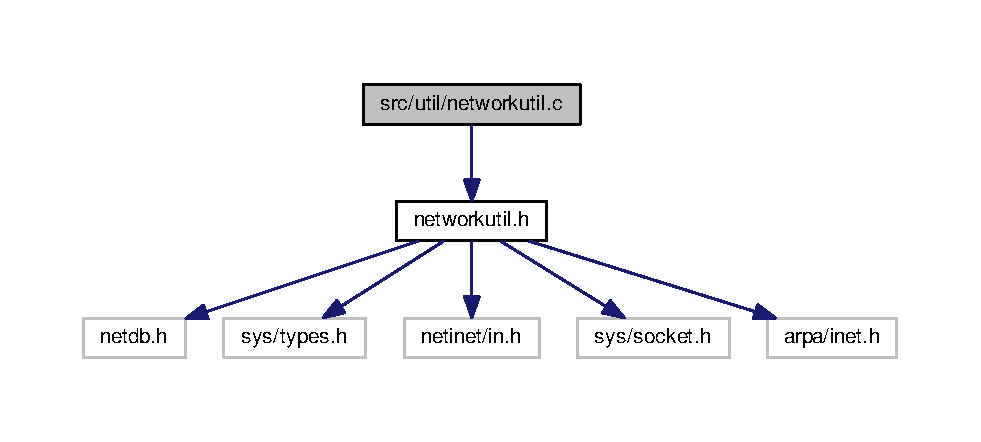
\includegraphics[width=350pt]{networkutil_8c__incl}
\end{center}
\end{figure}
\subsection*{Functions}
\begin{DoxyCompactItemize}
\item 
void $\ast$ \hyperlink{networkutil_8c_a294867ba9d7ff47e39d421134d8e12ab}{get\+\_\+in\+\_\+addr} (struct sockaddr $\ast$sa)
\begin{DoxyCompactList}\small\item\em Get the address structure correctly formatted\+: I\+Pv4 or I\+Pv6 from a generic {\ttfamily sockaddr} structure. \end{DoxyCompactList}\end{DoxyCompactItemize}


\subsection{Detailed Description}
Collection of utility methods used in the c-\/chat project. 

\begin{DoxyAuthor}{Author}
Enrico Vianello (\href{mailto:enrico.vianello.1@studenti.unipd.it}{\tt enrico.\+vianello.\+1@studenti.\+unipd.\+it}) 
\end{DoxyAuthor}
\begin{DoxyVersion}{Version}
1.\+0 
\end{DoxyVersion}
\begin{DoxySince}{Since}
1.\+0
\end{DoxySince}
\begin{DoxyCopyright}{Copyright}
Copyright (c) 2016-\/2017, Enrico Vianello 
\end{DoxyCopyright}


\subsection{Function Documentation}
\index{networkutil.\+c@{networkutil.\+c}!get\+\_\+in\+\_\+addr@{get\+\_\+in\+\_\+addr}}
\index{get\+\_\+in\+\_\+addr@{get\+\_\+in\+\_\+addr}!networkutil.\+c@{networkutil.\+c}}
\subsubsection[{\texorpdfstring{get\+\_\+in\+\_\+addr(struct sockaddr $\ast$sa)}{get_in_addr(struct sockaddr *sa)}}]{\setlength{\rightskip}{0pt plus 5cm}void$\ast$ get\+\_\+in\+\_\+addr (
\begin{DoxyParamCaption}
\item[{struct sockaddr $\ast$}]{sa}
\end{DoxyParamCaption}
)}\hypertarget{networkutil_8c_a294867ba9d7ff47e39d421134d8e12ab}{}\label{networkutil_8c_a294867ba9d7ff47e39d421134d8e12ab}


Get the address structure correctly formatted\+: I\+Pv4 or I\+Pv6 from a generic {\ttfamily sockaddr} structure. 


\begin{DoxyParams}{Parameters}
{\em sa} & The {\ttfamily sockaddr} struct.\\
\hline
\end{DoxyParams}
\begin{DoxyReturn}{Returns}
A pointer to a structure {\ttfamily sin\+\_\+addr} (if the address is I\+Pv4) or {\ttfamily sin6\+\_\+addr} (if the address is I\+Pv6). 
\end{DoxyReturn}

\hypertarget{networkutil_8h}{}\section{src/util/networkutil.h File Reference}
\label{networkutil_8h}\index{src/util/networkutil.\+h@{src/util/networkutil.\+h}}


Collection of utility methods used in the c-\/chat project.  


{\ttfamily \#include $<$netdb.\+h$>$}\\*
{\ttfamily \#include $<$sys/types.\+h$>$}\\*
{\ttfamily \#include $<$netinet/in.\+h$>$}\\*
{\ttfamily \#include $<$sys/socket.\+h$>$}\\*
{\ttfamily \#include $<$arpa/inet.\+h$>$}\\*
Include dependency graph for networkutil.\+h\+:\nopagebreak
\begin{figure}[H]
\begin{center}
\leavevmode
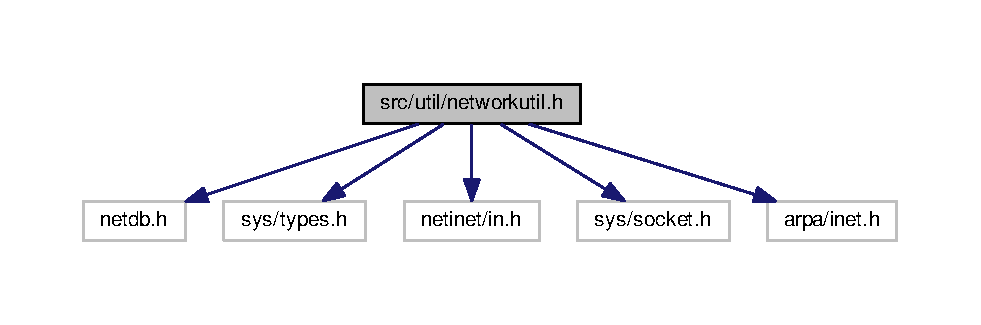
\includegraphics[width=350pt]{networkutil_8h__incl}
\end{center}
\end{figure}
This graph shows which files directly or indirectly include this file\+:\nopagebreak
\begin{figure}[H]
\begin{center}
\leavevmode
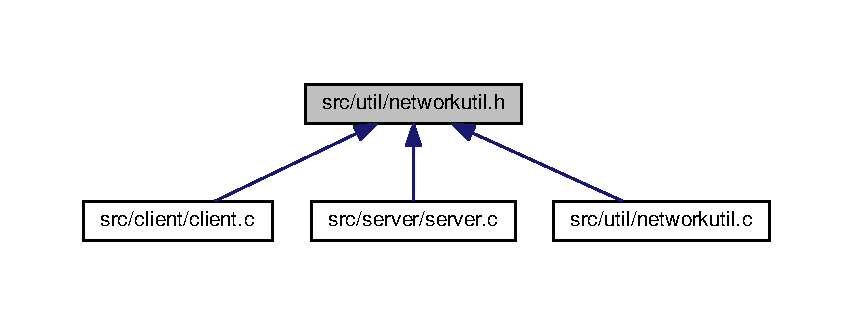
\includegraphics[width=350pt]{networkutil_8h__dep__incl}
\end{center}
\end{figure}
\subsection*{Functions}
\begin{DoxyCompactItemize}
\item 
void $\ast$ \hyperlink{networkutil_8h_a294867ba9d7ff47e39d421134d8e12ab}{get\+\_\+in\+\_\+addr} (struct sockaddr $\ast$sa)
\begin{DoxyCompactList}\small\item\em Get the address structure correctly formatted\+: I\+Pv4 or I\+Pv6 from a generic {\ttfamily sockaddr} structure. \end{DoxyCompactList}\end{DoxyCompactItemize}


\subsection{Detailed Description}
Collection of utility methods used in the c-\/chat project. 

\begin{DoxyAuthor}{Author}
Enrico Vianello (\href{mailto:enrico.vianello.1@studenti.unipd.it}{\tt enrico.\+vianello.\+1@studenti.\+unipd.\+it}) 
\end{DoxyAuthor}
\begin{DoxyVersion}{Version}
1.\+0 
\end{DoxyVersion}
\begin{DoxySince}{Since}
1.\+0
\end{DoxySince}
\begin{DoxyCopyright}{Copyright}
Copyright (c) 2016-\/2017, Enrico Vianello 
\end{DoxyCopyright}


\subsection{Function Documentation}
\index{networkutil.\+h@{networkutil.\+h}!get\+\_\+in\+\_\+addr@{get\+\_\+in\+\_\+addr}}
\index{get\+\_\+in\+\_\+addr@{get\+\_\+in\+\_\+addr}!networkutil.\+h@{networkutil.\+h}}
\subsubsection[{\texorpdfstring{get\+\_\+in\+\_\+addr(struct sockaddr $\ast$sa)}{get_in_addr(struct sockaddr *sa)}}]{\setlength{\rightskip}{0pt plus 5cm}void$\ast$ get\+\_\+in\+\_\+addr (
\begin{DoxyParamCaption}
\item[{struct sockaddr $\ast$}]{sa}
\end{DoxyParamCaption}
)}\hypertarget{networkutil_8h_a294867ba9d7ff47e39d421134d8e12ab}{}\label{networkutil_8h_a294867ba9d7ff47e39d421134d8e12ab}


Get the address structure correctly formatted\+: I\+Pv4 or I\+Pv6 from a generic {\ttfamily sockaddr} structure. 


\begin{DoxyParams}{Parameters}
{\em sa} & The {\ttfamily sockaddr} struct.\\
\hline
\end{DoxyParams}
\begin{DoxyReturn}{Returns}
A pointer to a structure {\ttfamily sin\+\_\+addr} (if the address is I\+Pv4) or {\ttfamily sin6\+\_\+addr} (if the address is I\+Pv6). 
\end{DoxyReturn}

%--- End generated contents ---

% Index
\backmatter
\newpage
\phantomsection
\clearemptydoublepage
\addcontentsline{toc}{chapter}{Index}
\printindex

\end{document}
